\chapter{การหาค่าดีที่สุด}
\label{chapter: Optimization}
\index{Optimization}
\index{การหาค่าดีที่สุด}


%\begin{verse}
%``Some progress quickly with a lot of pain, and others progress quickly with a lot of pleasure. It very much depends on our past accumulations of karma, how developed our spiritual faculties of mind already are. But if we’re facing in the right direction, all we have to do is keep on walking. If it takes a year, or sixty years, or five lifetimes, as long as we’re heading towards light, that’s all that matters.''
%Joseph Goldstein’s The Experience of Insight 
%\end{verse}

\begin{verse}
``... if we’re facing in the right direction, \\
all we have to do is keep on walking.'' \\
---Joseph Goldstein’s The Experience of Insight 
\end{verse}

\begin{verse}
``... ถ้าเรามุ่งหน้าไปในทิศทางที่ถูกต้อง \\
สิ่งที่เราต้องทำก็แค่เดินไปเรื่อยๆ'' \\
---ประสบการณ์แห่งความเข้าใจที่ลึกซึ้ง โจเซฟ โกล์ดสไตน์ 
\end{verse}

\textit{การเรียนรู้ของเครื่อง}ในมุมมองหนึ่งก็คือ\textit{การสร้างโมเดล}และ\textit{การหาค่าพารามิเตอร์ที่ดีที่สุด}ให้กับโมเดล โดยอาศัยประสบการณ์ที่เกี่ยวข้องช่วย.
การหาค่าพารามิเตอร์ที่ดีที่สุดสามารถใช้เทคนิคและความรู้จากศาสตร์และศิลป์ของวิชา\textit{การหาค่าดีที่สุด} (Optimization) มาช่วยได้.
วิชาการหาค่าดีที่สุดมีรายละเอียดมาก และด้วยเนื้อหาของวิชาการหาค่าดีที่สุดเองก็มากพอที่จะเป็นตำราของตัวเองได้.
บทนี้จะถกถึงเฉพาะพื้นฐานบางส่วนของศาสตร์การหาค่าดีที่สุดที่พอจะช่วยให้เข้าใจกระบวนการเกี่ยวข้องกับศาสตร์การเรียนรู้ของเครื่องบ้างเท่านั้น.

\section{การหาค่าดีที่สุดพื้นฐาน}
\label{section: Optimization}
\index{Optimization}
\index{การหาค่าดีที่สุด}

การหาค่าดีที่สุด (Optimization) คือการเลือกค่าของปัจจัย (แทนด้วยตัวแปร) ที่มีผลให้เป้าหมาย (แทนด้วยฟังชั่นของตัวแปร) มีค่าน้อย หรือมากที่สุด.
ปัจจัยที่ต้องการเลือก จะเรียกว่า \textit{ตัวแปรตัดสินใจ} (Decision Variable) และ
เป้าหมาย จะเรียกว่า \textit{ฟังชั่นจุดประสงค์} (Objective Function).
%
ตัวอย่างเช่น การเลือกเลือกค่าปัจจัยอุณหภูมิ แทนด้วยตัวแปร $x$ เพื่ออบมะเขือเทศได้อร่อยที่สุด โดยวัดจากปริมาณน้ำตาลที่ได้มากที่สุด โดยฟังชั่น $h$ แสดงความสัมพันธ์ระหว่างอุณหภูมิกับปริมาณน้ำตาลที่ได้จากการอบมะเขือเทศ.
ตัวแปร $x$ คือตัวแปรตัดสินใจ และฟังชั่น $h$ คือฟังชั่นจุดประสงค์.
กรณีนี้คือ การหาค่า $x$ ที่ทำให้ได้ค่าฟังชั่น $h$ มากที่สุด.
%ตัวอย่างเช่น การเลือกเลือกค่าตัวแปรนำ้หนัก $w_0$ กับ $w_1$ เพื่อให้ค่าความผิดพลาดจากการประมาณน้อยที่สุด.
%ตัวแปร $w_0$ กับ $w_1$ คือตัวแปรตัดสินใจ (ในกรณีนี้ มี $2$ ตัวแปร)
%และ\textit{ฟังชั่นค่าความผิดพลาด} (สมการ~\ref{eq: bg curve fitting E}) คือฟังชั่นจุดประสงค์.

ปัญหาที่เป็นการหาค่าที่ทำให้เป้าหมายมีค่ามากที่สุด เรียกรวมๆว่า \textit{ปัญหาค่ามากที่สุด} (Maximization Problem).
ตัวอย่างการเลือกอุณหภูมิการอบมะเขือเทศเพื่อให้ได้ปริมาณน้ำตาลสูงสุด เป็น\textit{ปัญหาค่ามากที่สุด}.
การเลือกชนิดการลงทุนเพื่อให้ได้ผลตอบแทนมากที่สุด 
การเลือกความเร็วของรถเพื่อวิ่งได้ระยะทางไกลที่สุด (ระยะทางมากที่สุด) สำหรับนำ้มัน $1$ ถัง 
เหล่านี้เป็นตัวอย่างของ\textit{ปัญหาค่ามากที่สุด}.

ทำนองเดียวกัน ปัญหาที่เป็นการหาค่าที่ทำให้เป้าหมายมีค่าน้อยที่สุด เรียกรวมๆว่า \textit{ปัญหาค่าน้อยที่สุด} (Minimization Problem).
ตัวอย่างเช่น การเลือกเส้นทางขับรถจากขอนแก่นไปร้อยเอ็ด โดยใช้เวลาเดินทางให้น้อยที่สุด.

ในทางคณิตศาสตร์ ปัญหาค่าน้อยที่สุดกับปัญหาค่ามากที่สุด สามารถแปลงไปมาระหว่างกันได้.
นั่นคือ การหาค่า $x$ ที่ทำให้ $h(x)$ มีค่ามากที่สุด 
จะเทียบเท่ากับ การหาค่า $x$ ที่ทำให้ $-h(x)$ มีค่าน้อยที่สุด (ดูแบบฝึกหัดการหาค่าดีที่สุด).
ดังนั้น เพื่อความสะดวก ปัญหาการหาค่าดีที่สุด ไม่ว่าจะเป็นปัญหาค่าน้อยที่สุดหรือปัญหาค่ามากที่สุด ก็สามารถเขียนให้อยู่ในรูปปัญหาค่าน้อยที่สุด ได้ดังนี้
\begin{eqnarray}
   \underset{\mathbf{x}}{\mbox{minimize}} & g(\mathbf{x})
\nonumber \\
   \mbox{subject to} & \mathbf{x} \in \Omega
\end{eqnarray}
โดย $\mathbf{x}$ คือตัวแปรตัดสินใจ (ซึ่งอาจมีหลายมิติ $\mathbf{x} = [x_1, x_2, \ldots, x_n]^T \in \mathbb{R}^n$),
$g: \mathbb{R}^n \to \mathbb{R}$ เป็นฟังชั่นจุดประสงค์ (หรือ Cost Function),
และเซต $\Omega$ เป็นซับเซตของ $\mathbb{R}^n$ ที่ระบุค่าของตัวแปรในช่วงที่สนใจหรือยอมรับได้ เรียกว่า เซตข้อจำกัด (Constraint Set หรือ Feasible Set).
ถ้า $\Omega = \mathbb{R}^n$ (หรือไม่มีข้อจำกัดของตัวแปรตัดสินใจ) จะเรียกปัญหาแบบนี้ว่า \textit{ปัญหาหาค่าดีที่สุดแบบไม่มีข้อจำกัด} (Unconstrained Optimization Problem).
เพื่อความสะดวก ค่าตัวแปรตัดสินใจที่ทำให้ฟังชั่นเป้าหมายมีค่าน้อยที่สุด จะเรียกว่า \textit{ค่าทำน้อยที่สุด} (Minimizer) และนิยมใช้ตัวยกดอกจันทร์ตามตัวแปร เช่น $\mathbf{x}^*$ เพื่อระบุว่า กำลังพูดถึง\textit{ค่าทำน้อยที่สุด}.

เมื่อพูดถึงการหาค่าน้อยที่สุด สิ่งที่ต้องการคือ ค่าทำน้อยที่สุดและค่าฟังชั่นเป้าหมายของมัน (ซึ่งน้อยที่สุด).
ค่าทำน้อยที่สุด มี $2$ ประเภท ได้แก่ ค่าทำน้อยที่สุดท้องถิ่น และ ค่าทำน้อยที่สุดทั่วหมด.

\paragraph{นิยามของค่าทำน้อยที่สุดท้องถิ่น.}
สมมติ $g: \mathbb{R}^n \to \mathbb{R}$ เป็นฟังชั่นค่าจริงที่นิยามสำหรับเซต $\Omega \subset \mathbb{R}^n$. 
จุด $\mathbf{x}^* \in \Omega$ เป็นค่าทำน้อยที่สุดท้องถิ่น (Local Minimizer) ของ $g$ บนเซต $\Omega$ ถ้ามีค่า $\epsilon > 0$ ที่ $g(\mathbf{x}) \geq f(\mathbf{x}^*)$ สำหรับ ทุกค่า $\mathbf{x} \in \Omega \setminus \{ \mathbf{x}^*\}$ และ $\| \mathbf{x} - \mathbf{x}^* \| < \epsilon$.

\paragraph{นิยามของค่าทำน้อยที่สุดทั่วหมด.}
จุด $\mathbf{x}^* \in \Omega$  เป็นค่าทำน้อยที่สุดทั่วหมด (Global Minimizer) ของฟังชั่น $g$ บนเซต $\Omega$ ถ้า $g(\mathbf{x}) \geq g(\mathbf{x}^*)$ สำหรับทุก $\mathbf{x} \in \Omega \setminus \{\mathbf{x}^*\}$.

จากนิยามข้างต้น กล่าวง่ายๆก็คือ 
\textit{ค่าทำน้อยที่สุดท้องถิ่น}คือค่าตัวแปรตัดสินใจที่ให้ค่าเป้าหมายน้อยกว่าค่าเป้าหมายบริเวณรอบๆ (ท้องถิ่น).
ส่วน \textit{ค่าทำน้อยที่สุดทั่วหมด}คือค่าตัวแปรตัดสินใจที่ให้ค่าเป้าหมายน้อยกว่าค่าเป้าหมายของทุกๆค่าตัวแปรตัดสินใจที่เป็นไปได้ (ทั่วทั้งหมด).
ดังนั้น \textit{ค่าทำน้อยที่สุดทั่วหมด} ก็จะเป็น\textit{ค่าทำน้อยที่สุดท้องถิ่น}ด้วยเสมอ.
รูป~\ref{fig: minimizers} แสดงค่าทำน้อยที่สุดต่างๆ โดย 
\texttt{x1} เป็นทั้งค่าทำน้อยที่สุดทั่วหมดและค่าทำน้อยที่สุดท้องถิ่น
ส่วน \texttt{x2} ถึง \texttt{x6} เป็นค่าทำน้อยที่สุดท้องถิ่น.

%
\begin{figure}
\begin{center}
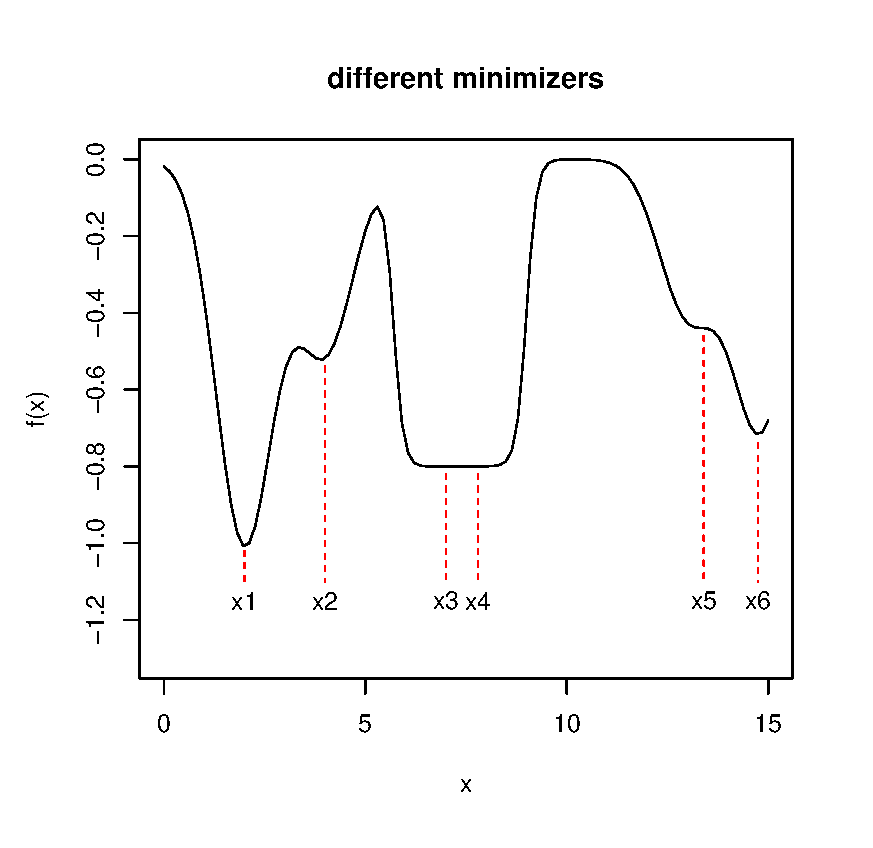
\includegraphics[height=3.0in]
{02Background/minimizers.eps}
\end{center}
\caption{ค่าทำน้อยที่สุดต่างๆ}
\label{fig: minimizers}
\end{figure}
%

\section{เงื่อนไขของค่าทำน้อยที่สุดท้องถิ่น}
\label{sec: opt FONC}

จากฟังชั่นเป้าหมาย $g: \mathbb{R}^n \mapsto \mathbb{R}$ อนุพันธ์อันดับหนึ่งของฟังชั่นเป้าหมาย เขียนย่อเป็น $D g$, คือ
\begin{eqnarray}
   D g = \left[ \frac{\partial g}{\partial x_1}, 
                \frac{\partial g}{\partial x_2},
                \ldots,
                \frac{\partial g}{\partial x_n}
         \right]
\end{eqnarray}
และเกรเดียนต์ (Gradient) $\nabla g = (D g)^T$.

อนุพันธ์อันดับสองของฟังชั่นเป้าหมาย เรียกว่า \textit{เฮเชียน} (Hessian of $g$) คือ
\begin{eqnarray}
   \mathbf{G}(\mathbf{x}) = D^2 g(\mathbf{x}) = 
   \begin{bmatrix}
   \frac{\partial^2 g}{\partial x_1^2} (\mathbf{x}) & \cdots & \frac{\partial^2 g}{\partial x_n x_1} (\mathbf{x}) \\
   \vdots    &        & \vdots \\
   \frac{\partial^2 g}{\partial x_1 x_n} (\mathbf{x}) & \cdots & \frac{\partial^2 g}{\partial x_n^2} (\mathbf{x})   
   \end{bmatrix}
\end{eqnarray}

\begin{myexample}
เช่น ถ้า $g(\mathbf{x}) = 2 x_1 + 18 x_2 + x_1 x_2 - x_1^2 - 4 x_2^2$, ดังนั้น
\begin{eqnarray}
   \nabla g (\mathbf{x}) = \begin{bmatrix}
   \frac{\partial g}{\partial x_1} (\mathbf{x}) \\
   \frac{\partial g}{\partial x_2} (\mathbf{x})   
   \end{bmatrix}
   = 
   \begin{bmatrix}
   2 + x_2 - 2 x_1 \\
   18 + x_1 - 8 x_2
   \end{bmatrix}   
\nonumber   
\end{eqnarray}
และ
\begin{eqnarray}
   \mathbf{G}(\mathbf{x}) = D^2 g(\mathbf{x}) = 
   \begin{bmatrix}
   \frac{\partial^2 g}{\partial x_1^2}(\mathbf{x}) & 
     \frac{\partial^2 g}{\partial x_2 x_1}(\mathbf{x}) \\
   \frac{\partial^2 g}{\partial x_1 x_2}(\mathbf{x}) & 
     \frac{\partial^2 g}{\partial x_2^2}(\mathbf{x})
   \end{bmatrix}
   = \begin{bmatrix}
   -2 & 1 \\
   1 & -8
   \end{bmatrix}
\nonumber
\end{eqnarray}
\end{myexample}


จากเซตข้อจำกัด $\Omega$ \textit{ค่าทำน้อยที่สุด}อาจจะอยู่ภายใน $\Omega$ (กรณีนี้เรียกว่า กรณีภายใน,  Interior Case) หรืออาจจะอยู่ที่ขอบของ $\Omega$ ก็ได้ (กรณีขอบเขต, Boundary Case).

เพื่อความสะดวกการศึกษาทั้งสองกรณี โดยเฉพาะกรณีขอบเขต เราจะนำแนวคิดของ\textit{ทิศทางซึ่งเป็นไปได้} 
(Feasible Direction) เข้ามา.

\paragraph{นิยามทิศทางซึ่งเป็นไปได้.}\index{ทิศทางซึ่งเป็นไปได้}\index{Feasible Direction}
เวกเตอร์ $\mathbf{d} \in \mathbb{R}^n, \mathbf{d} \neq \mathbf{0}$ เป็น\textit{ทิศทางซึ่งเป็นไปได้} 
(Feasible Direction) ที่ $\mathbf{x} \in \Omega$ ก็ต่อเมื่อมีค่า $\alpha_0 > 0$ ที่ทำให้ $\mathbf{x} + \alpha \mathbf{d} \in \Omega$ สำหรับทุกๆค่าของ $\alpha \in [0, \alpha_0]$.
%
ดูรูป~\ref{fig: feasible direction} และ \ref{fig: feasible directions at different points} ประกอบ.

%
\begin{figure}
\begin{center}
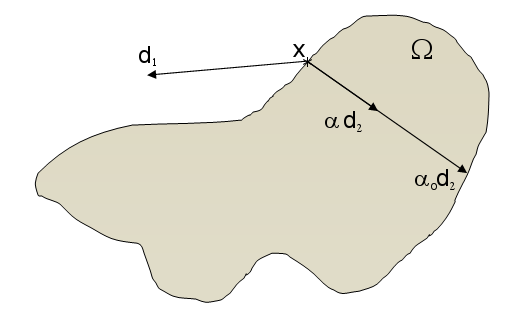
\includegraphics[width=2.0in]
{02Background/feasibleDirection01.png}
\end{center}
\caption{รูปประกอบช่วยอธิบาย\textit{ทิศทางซึ่งเป็นไปได้}. 
ทิศทาง $d_1$ ไม่ใช่\textit{ทิศทางซึ่งเป็นไปได้} 
ทิศทาง $d_2$ คือ\textit{ทิศทางซึ่งเป็นไปได้}ที่ $x$}
\label{fig: feasible direction}
\end{figure}
%


%
\begin{figure}
\begin{center}
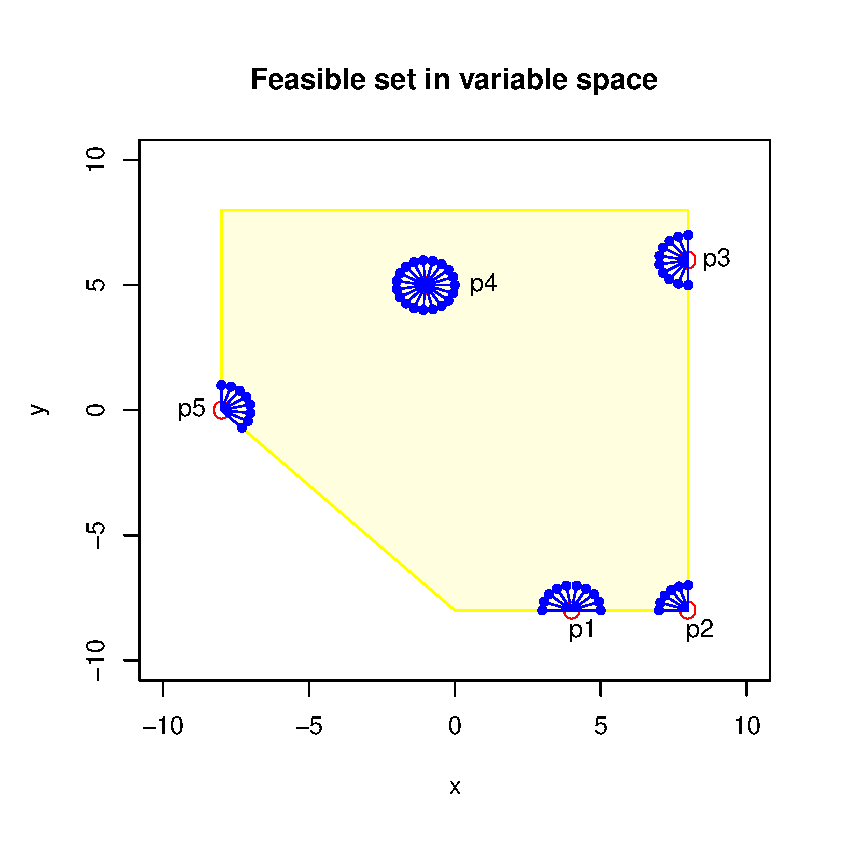
\includegraphics[width=4.0in]
{02Background/feasibleDirections.eps}
\end{center}
\caption{\textit{ทิศทางซึ่งเป็นไปได้}ที่จุดต่างๆ 5 จุด 
ได้แก่ \texttt{P1} ถึง \texttt{P5} ภายใน\textit{เซตข้อจำกัด} (ภายในพื้นที่แรเงา). เส้นเล็กที่วาดออกมาจากแต่ละจุด คือ ตัวอย่างของ\textit{ทิศทางซึ่งเป็นไปได้}ต่างๆที่จุดนั้น 
เช่นที่จุด \texttt{P1} ที่อยู่ชิดขอบล่างของ\textit{เซตข้อจำกัด} มี\textit{ทิศทางซึ่งเป็นไปได้}ต่างๆ ได้ตั้งแต่ทิศทางสามนาฬิกาทวนเข็มไปจนถึงเก้านาฬิกา).
สังเกตุ\textit{ทิศทางซึ่งเป็นไปได้}ต่างๆ ที่จุดที่อยู่ขอบของ\textit{เซตข้อจำกัด} (อาทิ จุด \texttt{P1}, \texttt{P2}, \texttt{P3}, \texttt{P5}) เทียบกับ จุด \texttt{P4} ที่อยู่ภายใน\textit{เซตข้อจำกัด}. 
หมายเหตุ เพื่อความสะดวกหัวเวกเตอร์วาดด้วยจุดแทนลูกศร}
\label{fig: feasible directions at different points}
\end{figure}
%

จากนิยาม\textit{ทิศทางซึ่งเป็นไปได้} เพื่อศึกษาคุณสมบัติหรือเงื่อนไขที่สามารถใช้ช่วยในการแก้ปัญหาการหาค่าน้อยที่สุด
พิจารณาการวิเคราะห์ต่อไปนี้.

ถ้าให้ ฟังชั่นค่าจริง $g: \mathbb{R}^n \mapsto \mathbb{R}$ และ $\mathbf{d}$ เป็น\textit{ทิศทางซึ่งเป็นไปได้}ที่ $\mathbf{x} \in \Omega$ แล้ว\textit{อนุพันธ์เชิงทิศทาง} (Directional Derivative) ของ $g$ ในทิศทาง $\mathbf{d}$ ซึ่งเขียนย่อด้วย $\partial g/\partial \mathbf{d}$, คือ
\begin{eqnarray}
   \frac{\partial g}{\partial \mathbf{d}} (\mathbf{x}) = \lim_{\alpha \to 0} \frac{g(\mathbf{x} + \alpha \mathbf{d}) - g(\mathbf{x})}{\alpha}.
\end{eqnarray}

ถ้า $\| d \| = 1$ แล้ว ค่า $\partial g/\partial \mathbf{d}$ ก็คือ อัตราการเพิ่มของค่าฟังชั่น $g$ ที่ $\mathbf{x}$ ในทิศทางของ $\mathbf{d}$ นั่นเอง.

สำหรับการคำนวณค่า $\partial g/\partial \mathbf{d}$ 
สมมติว่ามีค่า $\mathbf{x}$ กับ $\mathbf{d}$ อยู่ 
ดังนั้น $g(\mathbf{x} + \alpha \mathbf{d})$ เป็นฟังชั่นของ $\alpha$ หรือ
\begin{eqnarray}
   \frac{\partial g}{\partial \mathbf{d}} (\mathbf{x}) =
   \left. 
   \frac{d}{d \alpha} g(\mathbf{x} + \alpha \mathbf{d}) 
   \right|_{\alpha=0}
\nonumber
\end{eqnarray}
เมื่อใช้\textit{กฏลูกโซ่} (Chain Rule) เข้าไป จะได้
\begin{eqnarray}
\frac{d g(\mathbf{x} + \alpha \mathbf{d})}{d \alpha}
=
\frac{d g(\mathbf{x} + \alpha \mathbf{d})}{d (\mathbf{x} + \alpha \mathbf{d})} \cdot \frac{d (\mathbf{x} + \alpha \mathbf{d})}{d \alpha} 
%\nonumber \\
= (\nabla g(\mathbf{x})^T) \cdot (\mathbf{d}) = \mathbf{d}^T \nabla g(\mathbf{x}).
\nonumber
\end{eqnarray}

\paragraph{First-Order Necessary Condition (FONC).} \textit{เงื่อนไงจำเป็นอันดับแรก} (ของตัวทำต่ำสุด) คือ
ให้ $\Omega \subset \mathbb{R}^n$ และ $g \in \mathcal{C}^1$ เป็นฟังชั่นค่าจริงบนเซต $\Omega$ แล้ว
ถ้า $\mathbf{x}^*$ เป็น\textit{ตัวทำต่ำสุดท้องถิ่น}ของฟังชั่น $g$ บนเซต $\Omega$ แล้ว 
สำหรับแต่ละ\textit{ทิศทางซึ่งเป็นไปได้} $\mathbf{d}$ ที่ $\mathbf{x}^*$ ต้องได้ว่า
อนุพันธ์เชิงทิศทางที่จุดนั้นต้องมากกว่าหรือเท่ากับศูนย์. 
นั่นคือ
\begin{eqnarray}
   \mathbf{d}^T \nabla g(\mathbf{x}^*) \geq 0
\label{eq: FONC}
\end{eqnarray}
สำหรับทุกๆ $\mathbf{d}$.
%(ดูเพิ่มเติม โดยเฉพาะเรื่องพิสูจน์จาก \citet{ChongZak2ndEd}
หมายเหตุ $g \in \mathcal{C}^1$ หมายถึง ฟังชั่น $g$ เป็นฟังชั่นค่าต่อเนื่อง และมีอนุพันธ์อันดับหนึ่งทุกจุดบนเซตจำกัด.

รูป~\ref{fig: FONC} (รูปล่าง) แสดง\textit{ค่าทำน้อยที่สุด}ที่จุด \texttt{x1} (ที่ขอบซ้ายของเซตข้อจำกัด) พร้อมเกรเดียนต์ (\texttt{v1}) และตัวอย่าง\textit{ทิศทางซึ่งเป็นไปได้} (\texttt{d1} กับ \texttt{d2}) ซึ่งเมื่อตรวจคุณสมบัติจะได้ตาม\textit{เงื่อนไงจำเป็นอันดับแรก} (FONC).

เมื่อพิจารณาเปรียบเทียบกับจุด \texttt{x2} ที่ขอบขวาของเซตข้อจำกัด 
ที่จุด \texttt{x2} มีเกรเดียนต์ (\texttt{v2}) 
และตัวอย่าง\textit{ทิศทางซึ่งเป็นไปได้} (\texttt{d3}),
จุด \texttt{x2} ไม่ผ่าน\textit{เงื่อนไงจำเป็นอันดับแรก} เพราะมี\textit{ทิศทางซึ่งเป็นไปได้} \texttt{d3} ที่ทำให้ $\mathbf{d}_3 \nabla f(\mathbf{x}_2) < 0$ (สังเกตุ ทิศทางของเวกเตอร์ \texttt{v2} และ \texttt{d3}).
เมื่อไม่ผ่าน\textit{เงื่อนไงจำเป็นอันดับแรก} จึงมั่นใจได้ว่า จุด \texttt{x2} ไม่ใช่ค่าทำน้อยที่สุด.


%
\begin{figure}
\begin{center}
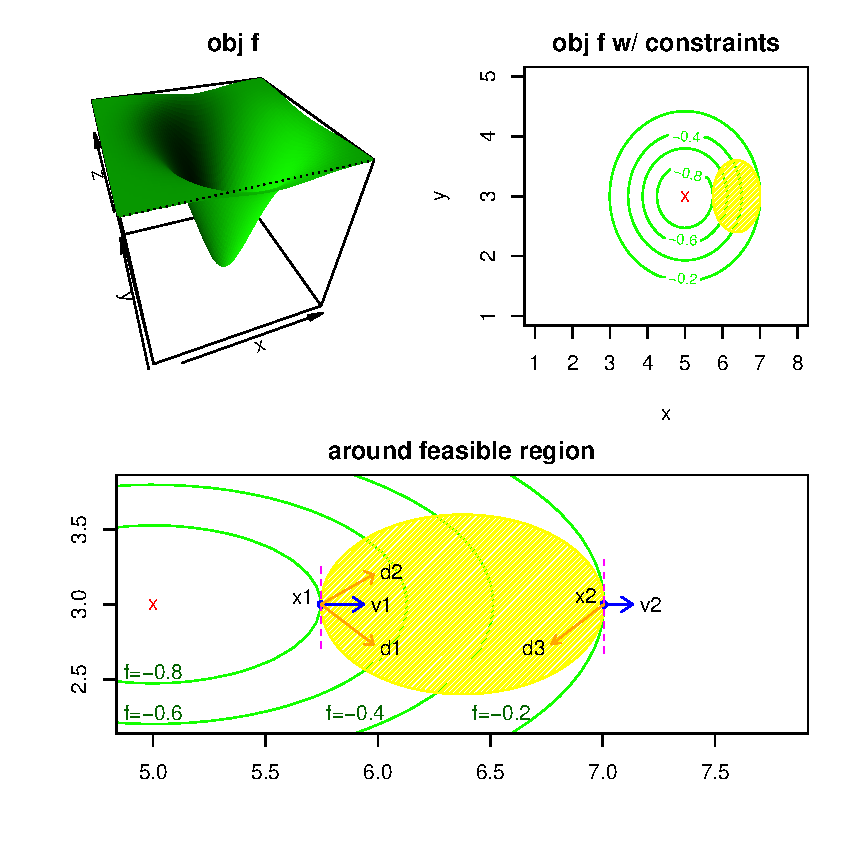
\includegraphics[width=6.0in]
{02Background/FONC.eps}
\end{center}
\caption{รูปบนซ้ายแสดงฟังชั่นเป้าหมายที่วาดแบบสามมิติ.
รูปบนขวาแสดงค่าฟังชั่นเป้าหมายที่วาดแบบคอนทัวร์ พร้อมแสดงเซตข้อจำกัด (พื้นที่ภายในวงกลมพื้นลาย), กากบาทสีแดงที่ $(5,3)$ คือ จุดที่ฟังชั่นเป้าหมายมีค่าน้อยที่สุด (แต่อยู่นอกเซตข้อจำกัด).
รูปล่างแสดงภาพขยายของรูปบนขวา โดยขยายเพื่อเน้นบริเวณเซตข้อกำจัด.
ที่จุด \texttt{x1} เป็น \textit{ค่าทำน้อยที่สุด}.
สังเกตุ ความสัมพันธ์ระหว่างเกรเดียนต์ (เวคเตอร์ \texttt{v}) กับทิศทางซึ่งเป็นไปได้ (เวคเตอร์ \texttt{d}) เปรียบเทียบความสัมพันธ์นี้ระหว่างจุด \texttt{x1} (ค่าทำน้อยที่สุด) กับ จุด \texttt{x2} ที่ขอบของเซตข้อจำกัดอีกด้าน}
\label{fig: FONC}
\end{figure}
%

\paragraph{เงื่อนไงจำเป็นอันดับแรกสำหรับกรณีภายใน.} 
ให้ $\Omega \subset \mathbb{R}^n$ และ $g \in \mathcal{C}^1$ เป็นฟังชั่นค่าจริงบนเซต $\Omega$ แล้ว
ถ้า $\mathbf{x}^*$ เป็น ตัวทำต่ำสุดของฟังชั่น $g$ บนเซต $\Omega$ และ ถ้า $\mathbf{x}^*$ เป็นจุดที่อยู่ภายในของเซต $\Omega$
% ($\mathbf{x}^*$ is an interior point) 
แล้วดังนั้น
\begin{eqnarray}
   \nabla g(\mathbf{x}^*) = \mathbf{0}.
\label{eq: FONC interior case}
\end{eqnarray}

%\begin{minipage}{5in}
%{\small
%\begin{shaded}
%\paragraph{ตัวอย่าง.}
\begin{myexample}
ปัญหาการค่าดีที่สุด
\begin{eqnarray}
  & \mbox{minimize}_{x_1, x_2} & 
     g(x_1, x_2) = x_1^2 + 0.5 x_2^2 + 3 x_2 + 73 
     \nonumber \\
  & \mbox{subject to } &
     x_1, x_2 \geq 0.
     \nonumber
\end{eqnarray}

รูป~\ref{fig: FONC example} แสดงค่าฟังชั่นเป้าหมายพร้อมขอบเขตของเซตข้อจำกัด.
ลองตรวจสอบเงื่อนไงจำเป็นอันดับแรกของจุด $(4,3), (3,0), (0,0)$ ดูว่าเป็นอย่างไรบ้าง.
ค่าเกรเดียนต์ คือ $\nabla g(\mathbf{x}) = [2 x_1 , x_2 + 3]^T$.
\begin{itemize}
\item ที่จุด $(4,3)$, $\nabla g(\mathbf{x} = [4,3]^T) = [2 x_1 , x_2 + 3]^T = [8, 6]^T$ และ ที่จุด $(4,3)$ (เป็นจุดภายใน, interior point), $\nabla g(\mathbf{x}) = [8, 6]^T \neq \mathbf{0}$  ดังนั้นจุดนี้จึงไม่ผ่านเงื่อนไงจำเป็นอันดับแรก.
% เราสามารถหา $\mathbf{d}$ ที่ทำให้ $\mathbf{d}^T \nabla f(\mathbf{x})$ ได้ เช่น $\mathbf{d} = [-1, 0]$, ดังนั้น จุด $(4,3)$ ไม่ผ่าน FONC.

\item ที่จุด $(3,0)$, $\nabla g(\mathbf{x} = [3,0]^T) = [6,3]^T$,
ดังนั้น $\mathbf{d}^T \nabla g(\mathbf{x}) = 6 d_1 + 3 d_2$ 
โดย $\mathbf{d} = [d_1, d_2]^T$.
ถ้าจะผ่านเงื่อนไงจำเป็นอันดับแรก ค่าของ $6 d_1 + 3 d_2$ ต้อง $\geq 0$ สำหรับทุกค่าของ $\mathbf{d}$ ที่จุด $(3,0)$ หรือ $6 d_1 + 3 d_2 \geq 0 \equiv d_1 \geq - d_2/2$.
แต่พบว่า มี\textit{ทิศทางซึ่งเป็นไปได้}ที่จุด $(3,0)$ 
เช่น $\mathbf{d} = [-1,0]^T$ จะทำให้ $\mathbf{d}^T \nabla f = -6 < 0$
ทำให้ จุด $(3,0)$ ไม่ผ่านเงื่อนไงจำเป็นอันดับแรก
%ที่ทำให้ $\mathbf{d}^T \nabla f < 0$ 
%ดังแสดงใน
ดูรูป~\ref{fig: FONC example P(3,0)} ประกอบ. %,  ไม่ผ่าน FONC.

\item ที่จุด $(0,0)$, $\nabla f(\mathbf{x} = [0,0]^T) = [0,3]^T$,
ดังนั้น $\mathbf{d}^T \nabla f(\mathbf{x}) = 3 d_2$, 
ซึ่งที่จุด $(0,0)$, $d_2 \geq 0$ จึงทำให้ $\mathbf{d}^T \nabla f(\mathbf{x}) \geq 0$ สำหรับทุกๆ\textit{ทิศทางซึ่งเป็นไปได้}.
จุด $(0,0)$ จึงผ่านเงื่อนไงจำเป็นอันดับแรก.
\end{itemize}

%\end{shaded}
%}%small
%\end{minipage}
\end{myexample}

%
\begin{figure}
\begin{center}
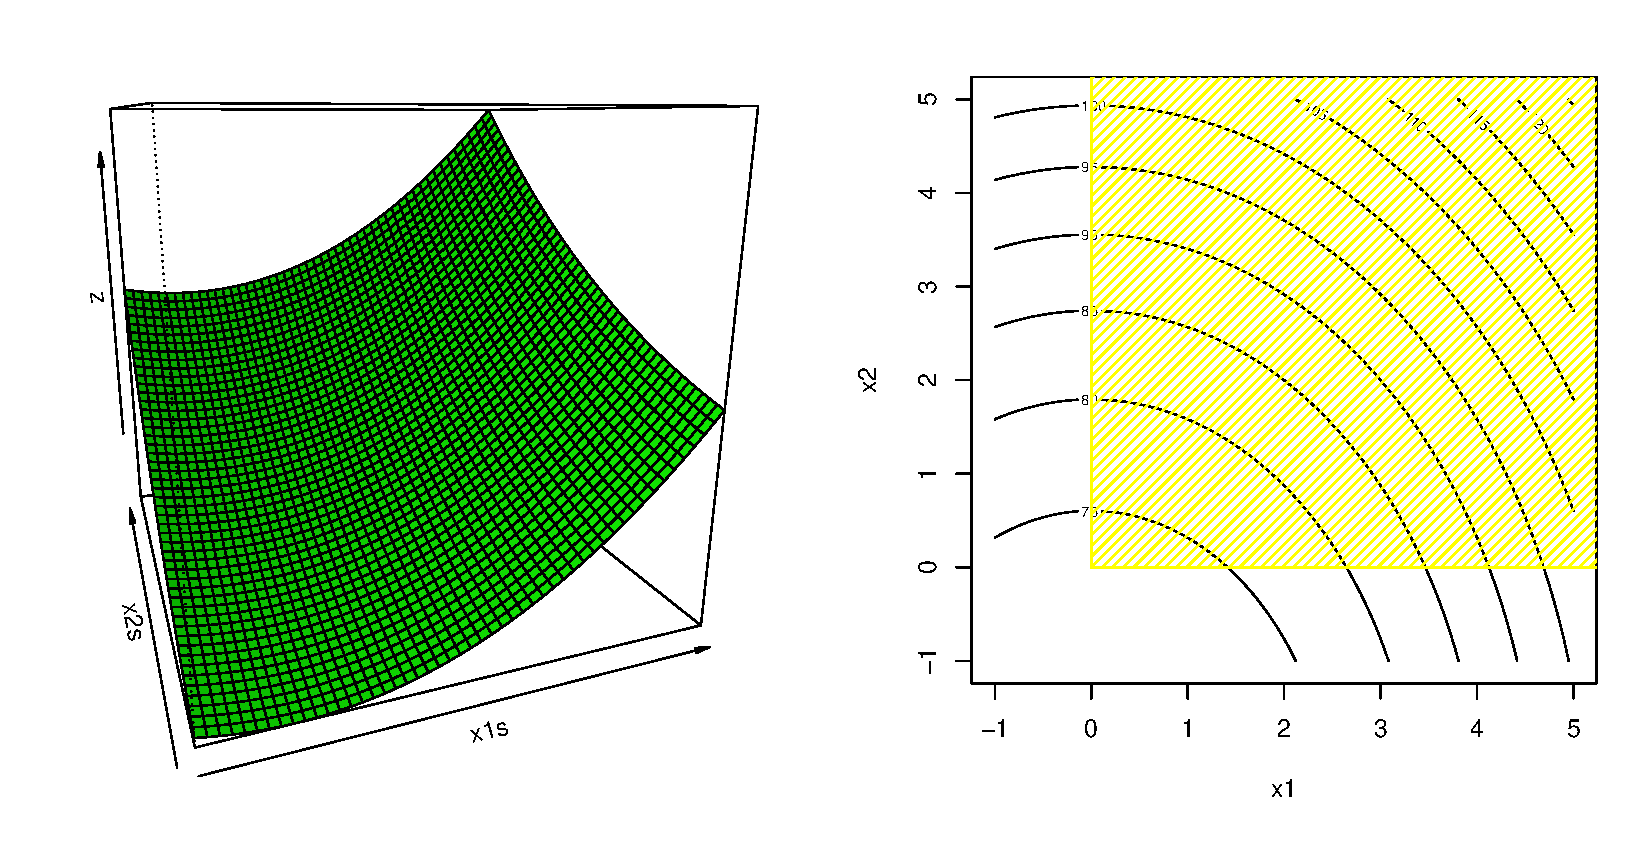
\includegraphics[width=6.0in]
{02Background/FONCexample.eps}
\end{center}
\caption{รูปซ้ายแสดงฟังชั่นเป้าหมายที่วาดแบบสามมิติ.
รูปบนขวาแสดงค่าฟังชั่นเป้าหมายที่วาดแบบคอนทัวร์ พร้อมเซตข้อจำกัด (พื้นที่แรเงา)}
\label{fig: FONC example}
\end{figure}
%


%
\begin{figure}
\begin{center}
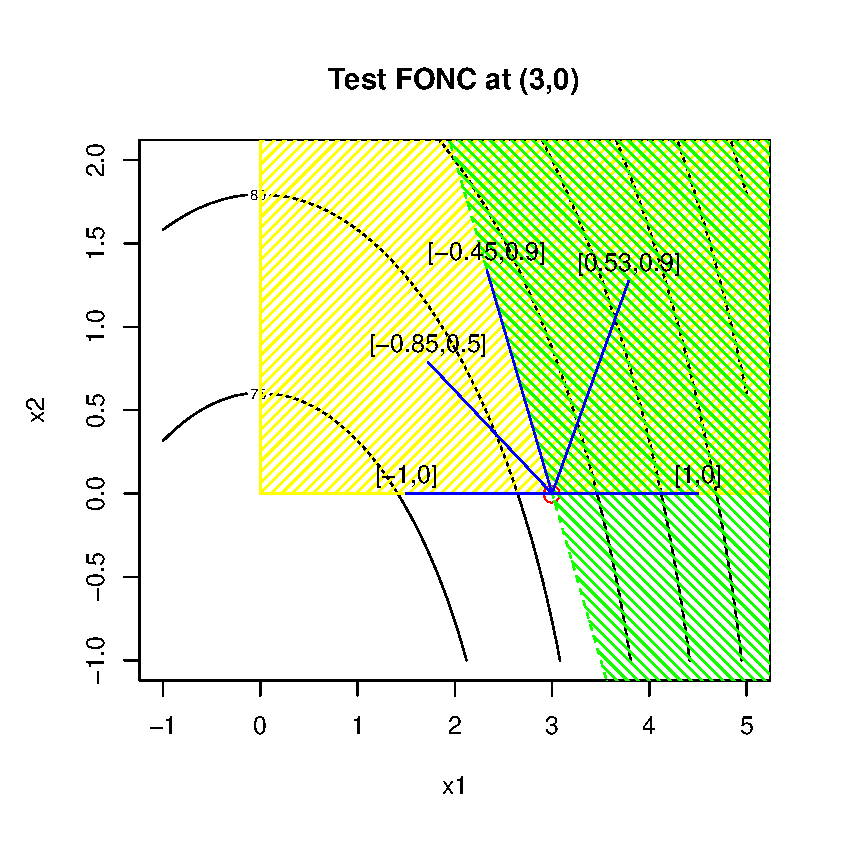
\includegraphics[width=4.0in]
{02Background/FONCExampleP30.eps}
\end{center}
\caption{ตัวอย่าง \textit{ทิศทางซึ่งเป็นไปได้}ที่จุด $(3,0)$.
ทิศทาง เช่น \texttt{[-1,0]} และ \texttt{[-0.85, 0.5]} 
จะทำให้ $\mathbf{d}^T \nabla f < 0$.}
\label{fig: FONC example P(3,0)}
\end{figure}
%

\paragraph{Second-Order Necessary Condition (SONC).} เงื่อนไขจำเป็นอันดับสอง (ของตัวทำต่ำสุด) คือ
ให้ $\Omega \subset \mathbb{R}^n$ และ $g \in \mathcal{C}^2$ เป็นฟังชั่นค่าจริงบนเซต $\Omega$,
ให้ $\mathbf{x}^*$ เป็น\textit{ตัวทำต่ำสุดท้องถิ่น}ของฟังชั่น $g$ บนเซต $\Omega$, สำหรับทุกๆ\textit{ทิศทางซึ่งเป็นไปได้} $\mathbf{d}$ ที่ $\mathbf{x}^*$, 
ถ้า $\mathbf{d}^T \nabla g(\mathbf{x}^*) = 0$, แล้ว
\begin{eqnarray}
   \mathbf{d}^T \mathbf{G}(\mathbf{x}^*) \mathbf{d} \geq 0,
\label{eq: SONC}
\end{eqnarray}
เมื่อ $\mathbf{G}$ เป็นเฮเชียนของ $g$.
หมายเหตุ $g \in \mathcal{C}^2$ หมายถึง ฟังชั่น $g$ เป็นฟังชั่นค่าต่อเนื่อง และมีอนุพันธ์อันดับสองทุกจุดบนเซตจำกัด (สามารถหาเฮเชียน $\mathbf{G}$ ได้).

\paragraph{เงื่อนไขจำเป็นอันดับสองสำหรับกรณีภายใน.} %SONC สำหรับ interior case}
ให้ $\mathbf{x}^*$ เป็นจุดที่อยู่ภายในเซตจำกัด $\Omega \subset \mathbb{R}^n$, ถ้า $\mathbf{x}^*$ เป็นตัวทำน้อยที่สุดท้องถิ่นของฟังชั่นเป้าหมาย $g: \Omega \to \mathbb{R}, g \in \mathcal{C}^2$, แล้ว
\begin{eqnarray}
   \nabla g(\mathbf{x}^*) = \mathbf{0},
\nonumber   
\end{eqnarray}
และ $\mathbf{G}(\mathbf{x}^*)$ เป็น\textit{บวกกึ่งแน่นอน} (Positive Semi-Definite, $\mathbf{G}(\mathbf{x}^*) \geq 0$) ซึ่งก็คือ
\begin{equation}
   \mathbf{d}^T \mathbf{G}(\mathbf{x}^*) \mathbf{d} \geq 0,
   \mbox{ for all } \mathbf{d} \in \mathbb{R}^n.   
\nonumber   
\end{equation}

%\begin{minipage}{5in}
%{\small
%\begin{shaded}
%\paragraph{ตัวอย่าง.}
\begin{myexample}
ฟังชั่นเป้าหมาย $g(x) = x^3$, ที่ $x = 0$ ค่า $g'(0) = 0$ และ $g''(0) = 0$ ดังนั้น ที่จุด $x = 0$ ผ่านทั้งเงื่อนไขจำเป็นอันดับหนึ่งและอันดับสอง.
แต่ $x=0$ ไม่ใช่ค่าทำน้อยที่สุด ดังแสดงในรูป~\ref{fig: x^3}.
%\end{shaded}
%}%small
%\end{minipage}
\end{myexample}

%
\begin{figure}
\begin{center}
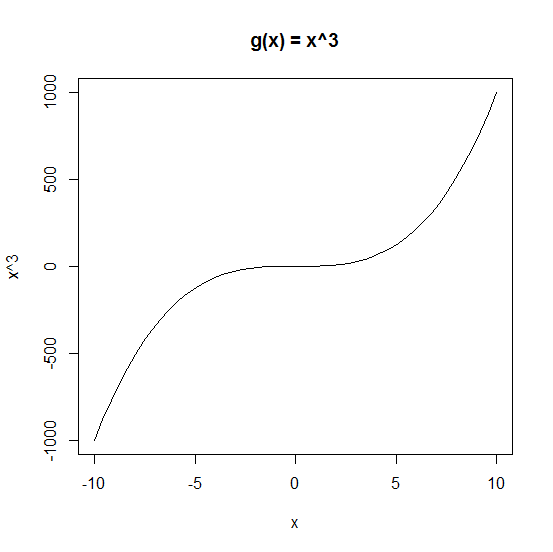
\includegraphics[width=4.0in]
{02Background/SONCexample01.png}
\end{center}
\caption{ตัวอย่าง ค่าฟังชั่น $g(x) = x^3$}
\label{fig: x^3}
\end{figure}
%

%\begin{minipage}{5in}
%{\small
%\begin{shaded}
%\paragraph{ตัวอย่าง.}
\begin{myexample}
ฟังชั่นเป้าหมาย $g(\mathbf{x}) = x_1^2 - x_2^2$ มีเกรเดียนต์ $\nabla g(\mathbf{x}) = [2 x_1, -2 x_2]^T$ และ เฮเชียน 
\begin{eqnarray}
   \mathbf{G}(\mathbf{x}) = \begin{bmatrix}
      2 & 0 \\
      0 & -2
   \end{bmatrix}.
\nonumber   
\end{eqnarray}

ที่ $\mathbf{x} = [0,0]^T$, $\nabla g(\mathbf{x}) = \mathbf{0}$ ซึ่งผ่านเงื่อนไขจำเป็นอันดับหนึ่ง 
แต่ค่าเฮเชียนไม่ได้เป็น\textit{บวกกึ่งแน่นอน} 
เนื่องจาก มี\textit{ทิศทางซึ่งเป็นไปได้} ที่ทำให้ $\mathbf{d}^T \mathbf{G} \mathbf{d} < 0$ 
เช่น $\mathbf{d} = [0,1]^T$.
จุด $\mathbf{x} = [0,0]^T$ จึงไม่ผ่านเงื่อนไขจำเป็นอันดับสอง ซึ่งยืนยันว่าจุดนี้ไม่ใช่ตัวทำน้อยที่สุด.
รูป~\ref{fig: SONC example} แสดงค่าฟังชั่นเป้าหมายของตัวอย่างนี้.
%\end{shaded}
%}%small
%\end{minipage}

\end{myexample}

%
\begin{figure}
\begin{center}
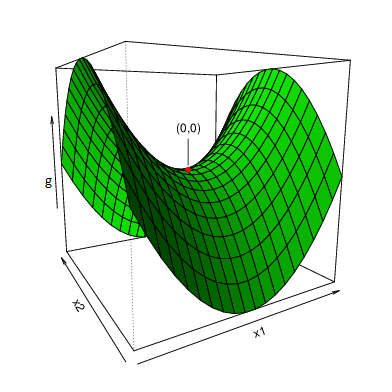
\includegraphics[width=4.0in]
{02Background/SONCexample02.png}
\end{center}
\caption{ตัวอย่างค่าฟังชั่น $g(x) = x_1^2 - x_2^2$.
แกนตั้งเป็นค่าฟังชั่น $g(x)$.
จุด $(0,0)$ ผ่านเงื่อนไขจำเป็นอันดับหนึ่ง แต่ไม่ผ่านเงื่อนไขจำเป็นอันดับสอง.}
\label{fig: SONC example}
\end{figure}
%

สังเกตุว่า ถ้าจุดใดไม่ผ่านเงื่อนไขจำเป็น จุดนั้นไม่ใช่ตัวทำต่ำสุด.
แต่จุดที่ผ่านเงื่อนไขจำเป็น จุดนั้นอาจจะไม่ใช่ตัวทำต่ำสุดก็ได้.

\paragraph{Second-Order Sufficient Condition (SOSC), Interior Case} 
เงื่อนไขเพียงพออันดับสอง สำหรับกรณีภายใน คือ
ให้ $g \in \mathcal{C}^2$ และ $\mathbf{x}^*$ เป็นจุดที่อยู่ภายในเซตข้อจำกัด,
ถ้า $\nabla g(\mathbf{x}^*) = \mathbf{0}$ และ 
$\mathbf{G}(\mathbf{x}^*) > 0$ แล้ว $\mathbf{x}^*$ เป็นตัวทำน้อยสุดท้องถิ่นอย่างแท้จริง (Strict Local Minimizer) ของ $g$.

%\begin{minipage}{5in}
%{\small
%\begin{shaded}
%\paragraph{ตัวอย่าง.}
\begin{myexample}
ฟังชั่นเป้าหมาย $g(\mathbf{x}) = x_1^2 + x_2^2$, เกรเดียนต์ $\nabla g(\mathbf{x}) = [2 x_1, 2 x_2]^T$ 
และค่าเกรเดียนต์ จะเท่ากับ $\mathbf{0}$ ก็เมื่อ $\mathbf{x} = [0,0]^T$ เท่านั้น 
และเนื่องจากค่าเฮเชียนเป็น
\begin{eqnarray}
   \mathbf{G}(\mathbf{x}) = \begin{bmatrix}
      2 & 0 \\
      0 & 2
   \end{bmatrix}
\nonumber   
\end{eqnarray}
ซึ่งเป็น\textit{บวกแน่นอน} ($\mathbf{G} > 0$) เพราะ 
$\mathbf{d}^T \mathbf{G} \mathbf{d} = 2 d_1^2 + 2 d_2^2 > 0$ ไม่ว่าค่า $d_1$ หรือ $d_2$ จะเป็นอะไร ($d_1, d_2 \in \mathbb{R}$).
จุด $(0,0)$ ผ่านเงื่อนไขทั้งเงื่อนไขจำเป็นอันดับหนึ่ง อันดับสอง และเงื่อนไขเพียงพออันดับสอง, จุด $(0,0)$ จึงเป็น\textit{ตัวทำค่าน้อยที่สุด}ของฟังชั่นนี้ (รูป~\ref{fig: SOSC example} แสดงฟังชั่นเป้าหมาย และจุด $(0,0)$).
%\end{shaded}
%}%small
%\end{minipage}
\end{myexample}

%
\begin{figure}
\begin{center}
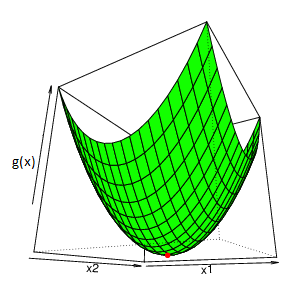
\includegraphics[width=4.0in]
{02Background/SOSC.png}
\end{center}
\caption{ตัวอย่าง ค่าฟังชั่น $g(x) = x_1^2 + x_2^2$.
แกนตั้งแทน $g(x)$.
จุด $(0,0)$ ผ่านทั้งเงื่อนไขจำเป็นอันดับหนึ่ง อันดับสอง และเงื่อนไขเพียงพออันดับสอง}
\label{fig: SOSC example}
\end{figure}
%

วิธีการหาค่าดีที่สุดมีหลายวิธี เนื้อหาของการหาค่าดีที่สุดมีมาก.
บทนี้อภิปรายเพียงบางวิธีเท่านั้น เพื่อผู้อ่านจะพอได้เห็นภาพคร่าวๆว่า ศาสตร์การหาค่าดีที่สุดมีวิธีการทำอย่างไรบ้าง.
%เราจะลองดูวิธีการหาค่าน้อยที่สุดแบบไม่มีข้อจำกัดก่อน แล้วค่อยดูวิธีที่จะจัดการกับข้อจำกัดใน หัวข้อ~\ref{sec: constraint optimization}.

\section{การค้นหาแบ่งช่วงทองคำ}
\label{sec: golden section search}
\index{Golden Section Search}
\index{การค้นหาแบ่งช่วงทองคำ}
\index{Line Search}

การค้นหาแบ่งช่วงทองคำ (Golden Section Search) เป็นหนึ่งในวิธี\textit{การค้นหาตามแนวเส้น} (Line Search) ที่ใช้หาค่าทำน้อยที่สุดสำหรับฟังชั่นเป้าหมาย $g: [a_0,b_0] \to \mathbb{R}$ โดย $[a_0,b_0] \subset \mathbb{R}$ และฟังชั่นเป้าหมาย $g$ เป็น\textit{ฐานนิยมเดี่ยว} (Unimodal, ซึ่งหมายความว่า ฟังชั่น $g$ มี\textit{ค่าทำน้อยที่สุดท้องถิ่น}ค่าเดียว (มีหลุมเดียว) ดูรูป~\ref{fig: unimodal} ประกอบ)

แนวคิดของวิธีค้นหาแบ่งช่วงทองคำ คือ 
เริ่มต้นจากช่วง $[a_0, b_0]$ แล้วจะเลือกประเมินค่าของฟังชั่นเป้าหมายบางจุด โดยพยายามจะทำการประเมินให้น้อยที่สุด.
จากจุดที่ประเมินค่า เราจะขยับช่วง $[a_0, b_0]$ ให้แคบลง และจะทำแบบนี้ไปจนในที่สุดได้ช่วงที่แคบพอ และก็จะได้ค่าทำน้อยที่สุดตามความแม่นยำที่ต้องการ.

เพื่อจะขยับช่วงให้แคบลง เราต้องรู้ค่าของฟังชั่นระหว่างช่วงอย่างน้อย $2$ ค่า เรียกว่า ค่า $g_a$ กับค่า $g_b$ แทนค่าฟังชั่นเป้าหมายที่จุด $a_1$ กับที่จุด $b_1$ ตามลำดับ.
ดูรูป~\ref{fig: golden section idea} ประกอบ.
สำหรับฟังชั่น\textit{ฐานนิยมเดี่ยว} ถ้าค่าฟังชั่น $g_a < g_b$ (สองภาพบนของรูป~ \ref{fig: golden section idea}) สิ่งที่บอกได้คือ ค่าทำน้อยที่สุดอาจอยู่ระหว่างช่วงย่อย $[a_0,a_1]$ (กรณีภาพบนซ้าย) 
หรือระหว่างช่วงย่อย $[a_1, b_1]$ (กรณีภาพบนขวา) 
แต่ไม่อยู่ระหว่างช่วงย่อย $[b_1, b_0]$ แน่ๆ 
(เพราะ ถ้าค่าทำน้อยที่สุดอาจอยู่ระหว่างช่วงย่อย $[b_1, b_0]$ 
ฟังชั่น $g(x)$ ก็ไม่ใช่\textit{ฐานนิยมเดี่ยว}).
ดังนั้นถ้าหากรู้ว่า $g_a < g_b$ เราสามารถทำช่วงให้แคบลงได้โดยตัดช่วงย่อย $[b_1, b_0]$ ออก.
ทำนองเดียวกัน ถ้าค่าฟังชั่น $g_a > g_b$ ก็บอกได้ว่าค่าทำน้อยที่สุดไม่อยู่ระหว่างช่วงย่อย $[a_0,a_1]$ แน่ๆ
และก็สามารถตัดช่วงย่อย $[a_0, a_1]$ ออกได้.
เราก็สามารถทำแบบนี้ซ้ำได้จนกว่าจะได้ช่วงที่แคบพอที่จะได้ค่าความแม่นยำที่ต้องการ.

\textit{วิธีค้นหาแบ่งช่วงทองคำ}จะทำการแบ่งอย่างสมมาตร.
นั่นคือ ช่วงย่อยด้านซ้ายกับช่วงย่อยด้านขวายาวเท่าๆกัน แต่ไม่เกยกัน
\begin{equation}
   a_1 - a_0 = b_0 - b_1 = \rho (b_0 - a_0)
\end{equation}
โดยที่ $\rho < \frac{1}{2}$.
เงื่อนไขของ $\rho$ มีเพื่อป้องกันไม่ให้ช่วงย่อย $[a_0,a_1]$ เกยกับช่วงย่อย $[b_1, b_0]$.
ดูรูป~\ref{fig: golden section sectioning} ประกอบ.

การเลือกค่าของอัตราส่วน $\rho$ จะเลือกค่าที่ทำให้เวลาขยับช่วงเข้าไปแล้ว สามารถช่วยประหยัดการคำนวณได้บ้าง ดังแสดงในรูป~\ref{fig: CZ7p3}
จากขั้นตอนที่ 1, เรามีค่าฟังชั่นที่จุด $a_1$ ซึ่งคือ $g_a^{(1)}$ กับค่าฟังชั่นที่จุด $b_1$ ซึ่วคือ $g_b^{(1)}$ อยู่%
\footnote{ตัวยก $\cdot^{(n)}$ ระบุว่าเป็นค่าที่ได้ในขั้นตอนที่ $n$}
หลังจากเปรียบเทียบแล้ว หากพบว่า $g_a^{(1)} < g_b^{(1)}$, สามารถขยับช่วงเข้ามาได้ 
โดยให้ $b_0^{(2)} = b_1^{(1)}$.
ถ้าการเลือกค่าของ $\rho$ ทำให้ $b_1^{(2)}$ ไปตรงกับ $a_1^{(1)}$ ได้ จะช่วยทำให้ในขั้นตอนที่ 2 ต้องการคำนวณแค่ค่าฟังชั่นที่ $a_1^{(2)}$ ไม่จำเป็นต้องคำนวณค่าที่ $b_1^{(2)}$ อีก เพราะว่าสามารถใช้ $g_b^{(2)} = g_a^{(1)}$ ได้เลย.

ดังนั้น เมื่อพิจารณาจาก $\rho (b_0^{(2)} - a_0^{(2)}) = b_0^{(2)} - b_1^{(2)}$ และ การพิจารณาสัดส่วนต่างๆในเทอมของ $\rho$ (ดูรูป~\ref{fig: golden search rho} ประกอบ) เราจะพบว่า
\begin{eqnarray}
  \rho (b_1^{(1)} - a_0^{(1)}) &=& b_1^{(1)} - a_1^{(1)}.
\label{eq: golden sec rho origin} 
\end{eqnarray}

เพื่อความกระทัดรัด สมมติ $b_0^{(1)} - a_0^{(1)} = L_1 = 1$
ดังนั้น $b_1^{(1)} - a_0^{(1)} = 1 - \rho$ และ $b_1^{(1)} - a_1^{(1)} = 1 - 2 \rho$
และแทนความสัมพันธ์เหล่านี้เข้าไปในสมการ~\ref{eq: golden sec rho origin} เราจะได้ว่า
\begin{eqnarray}
   \rho (1 - \rho) &=& 1 - 2 \rho
\nonumber \\
   \rho^2 - 3 \rho + 1 &=& 0
\nonumber
\end{eqnarray}
ซึ่งเมื่อแก้สมการหาค่า $\rho$ แล้วจะได้
\begin{eqnarray}
   \rho_1 &=& \frac{3 + \sqrt{5}}{2} \approx 2.618
\nonumber \\   
   \rho_2 &=& \frac{3 - \sqrt{5}}{2} \approx 0.382
\end{eqnarray}
แต่จากเงื่อนไขที่ต้องการ $\rho < 0.5$ (เพื่อไม่ให้ช่วงย่อยเกยกัน), 
ดังนั้นจึงได้ว่า $\rho = 0.382$.
สัดส่วนนี้จะตรงกับสิ่งที่นักเรขาคณิตกรีกโบราณศึกษา และเรียกว่า \textit{สัดส่วนทองคำ} (Golden Section).

%
\begin{figure}
\begin{center}
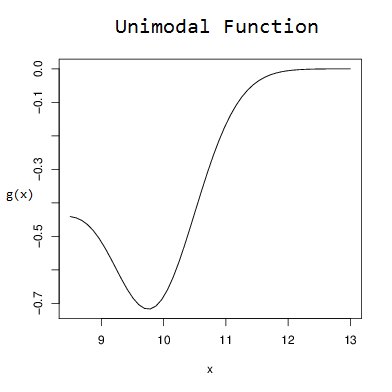
\includegraphics[width=4.0in]
{02Background/unimodal.png}
\end{center}
\caption{ตัวอย่างแสดงฟังชั่น\textit{ฐานนิยมเดี่ยว}}
\label{fig: unimodal}
\end{figure}
%

%
\begin{figure}
\begin{center}
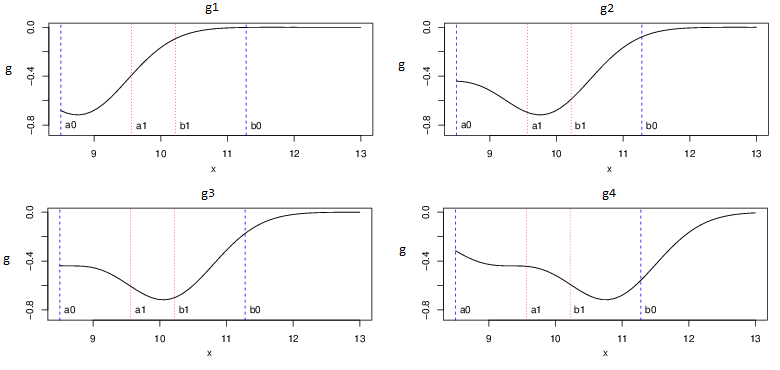
\includegraphics[width=6.0in]
{02Background/goldenSectionIdea.png}
\end{center}
\caption{ตัวอย่างแสดงแนวคิดของการขยับช่วงเข้าโดยดูจากค่าฟังชั่นระหว่างช่วงสองค่า.
ภาพซ้ายบน $g_a=g_1(a_1) < g_b=g_1(b_1)$ ส่อนัยว่าค่าทำน้อยที่สุดไม่อยู่ในช่วงย่อย $[b_1, b_0]$
เพราะว่า ค่า $g_1(b) \geq g_b,$ สำหรับทุกๆค่าของ $b \in [b_1, b_0]$. (เนื่องจาก $g_1$ เป็น\textit{ฐานนิยม}, มีหลุมเดียว.)
ภาพขวาบน $g_a=g_2(a_1) < g_b=g_2(b_1)$ ส่อนัยว่าค่าทำน้อยที่สุดไม่อยู่ในช่วงย่อย $[b_1, b_0]$.
หากเปรียบเทียบ ภาพซ้ายบนกับภาพขวาบน จะเห็นว่า เมื่อ $g_a < g_b$ ค่าทำน้อยที่สุดอาจจะอยู่ช่วง $[a_0, a_1]$ (กรณี $g_1$) หรืออาจจะอยู่ช่วง $[a_1, b_1]$ (กรณี $g_2$) ก็ได้.
แต่ค่าทำน้อยที่สุดไม่อยู่ในช่วงย่อย $[b_1, b_0]$ แน่ๆ.
ภาพซ้ายล่าง และภาพขวาล่าง แสดงสถานะการณ์ตัวอย่างเมื่อ $g_a > g_b$ ว่าอาจเป็นกรณี $g_3$ หรือ กรณี $g_4$ ก็ได้ แต่ที่รู้แน่ๆคือ ไม่ว่าจะเป็นกรณี $g_3$ หรือกรณี $g_4$ ค่าทำน้อยที่สุดก็ไม่อยู่ในช่วงย่อย $[a_0, a_1]$.
}
\label{fig: golden section idea}
\end{figure}
%

%
\begin{figure}
\begin{center}
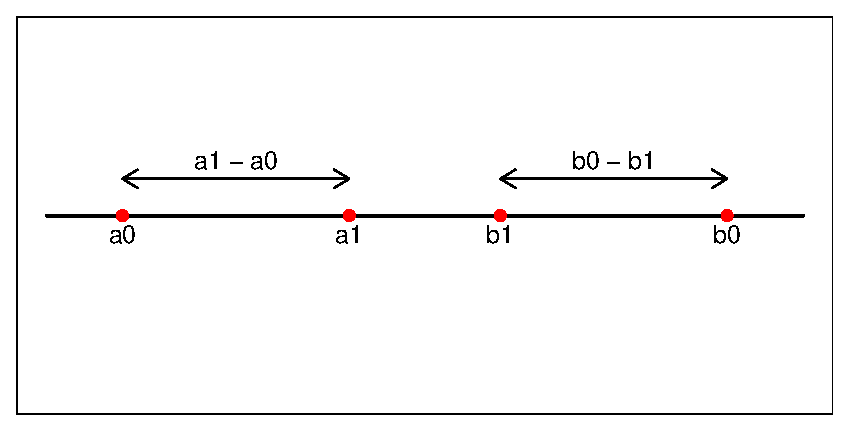
\includegraphics[width=4.0in]
{02Background/goldsecSectioning.eps}
\end{center}
\caption{การแบ่งส่วนจากช่วงที่สนใจ}
\label{fig: golden section sectioning}
\end{figure}
%

%
\begin{figure}
\begin{center}
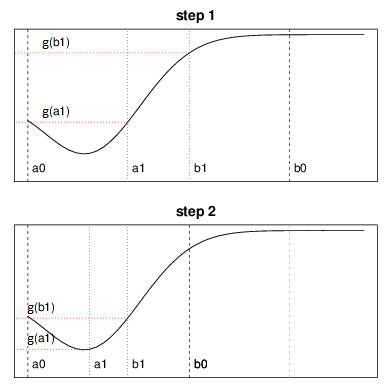
\includegraphics[width=5.0in]
{02Background/CZ7p3.png}
\end{center}
\caption{การขยับช่วงโดยจัดอัตราส่วน $\rho$ ให้พอดีช่วงจะช่วยประหยัดการคำนวณค่าฟังชั่นได้.
ตัวอย่าง เช่น ค่า $g_b$ ในขั้นตอนที่ 2 จะเท่ากับค่า $g_a$ จากขั้นตอนที่ 1 จะช่วยประหยัดไม่ต้องทำการคำนวณ $g(b_1)$ อีก}
\label{fig: CZ7p3}
\end{figure}
%

%
\begin{figure}
\begin{center}
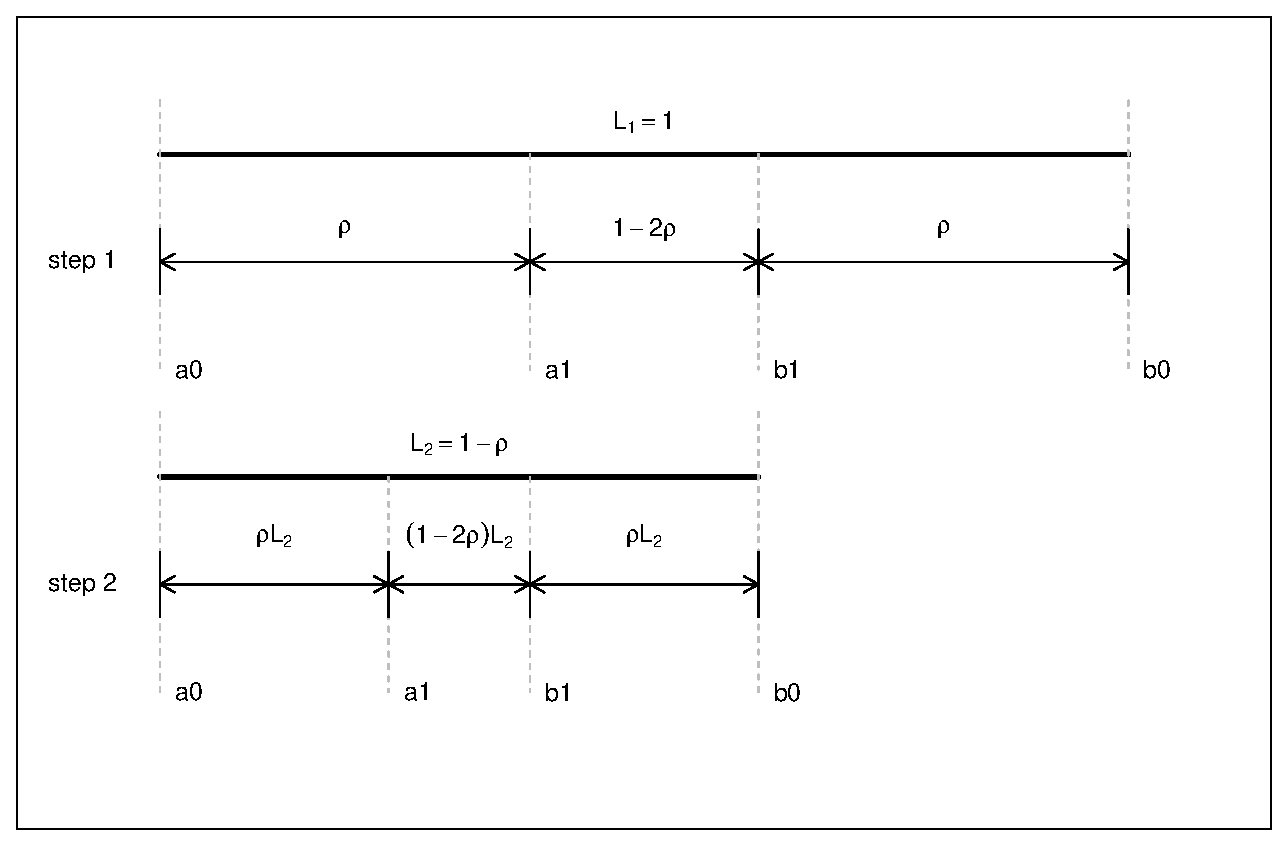
\includegraphics[width=6.0in]
{02Background/goldsecRho.eps}
\end{center}
\caption{สัดส่วนต่างๆในเทอมของ $\rho$.
สังเกตุว่า หากต้องการจัดการคำนวณให้มีประสิทธิภาพ กรณีนี้ $a_0^{(2)} = a_0^{(1)}$, $a_1^{(2)}$ เป็นจุดใหม่, $b_1^{(2)}=a_1^{(1)}$ และ $b_0^{(2)} = b_1^{(1)}$.
หากจัดสัดส่วนแบบนี้แล้ว ช่วยให้แต่ละขั้นตอนของการคำนวณมีจุดที่ต้องคำนวณใหม่เพียงจุดเดียว.
ค่า $\rho$ สามารถพิจารณาคำนวณได้จากความสัมพันธ์ $\rho (b_0^{(2)} - a_0^{(2)}) = b_0^{(2)} - b_1^{(2)} \Rightarrow \rho (b_1^{(1)} - a_0^{(1)}) = b_1^{(1)} - a_1^{(1)}$.}
\label{fig: golden search rho}
\end{figure}
%

ขนาดช่วงของตัวแปรจะลดลงในอัตราส่วน $1-\rho \approx 0.61803$ ต่อการทำแบ่งช่วงทองคำ $1$ ขั้นตอน เพราะฉะนั้นถ้าทำ $N$ ขั้นตอน ขนาดช่วงจะแคบเป็น $(1-\rho)^N \approx (0.61803)^N$ เท่าของช่วงเริ่มต้น.

%\begin{minipage}{5in}
%{\small
%\begin{shaded}
\begin{myexample}
%\paragraph{ตัวอย่าง.}
การใช้การค้นหาแบ่งช่วงทองคำ เพื่อหาค่าทำน้อยที่สุดของฟังชั่น $g(x) = -0.4 \exp(-(x-8)^2)-0.7 \exp(-(x-9.8)^2)$ ภายในช่วง $[8.5, 13]$.
สมมติหากต้องการความแม่นยำของคำตอบให้มีค่าน้อยกว่า $1$, จะต้องทำการค้นหาแบ่งช่วงทองคำ $N$ ขั้นตอน
โดย $(13 - 8.5) \cdot (0.61803)^N < 1$,
ซึ่งถ้า $N = 3$, จะได้ขนาดช่วงสุดท้ายเป็น $1.0623$ และถ้า $N = 4$, จะได้ขนาดช่วงสุดท้ายเป็น $0.6565$ เพราะฉะนั้นหากต้องการค่าความแม่นยำน้อยกว่า $1$ จะทำ $4$ ขั้นตอน.
รูป~\ref{fig: golden search example} แสดงภาพประกอบของ.

\begin{itemize}
\item ขั้น $1$, $a_0 = 8.5$ และ $b_0 = 13$, ดังนั้น $a_1 = a_0 + (b_0 - a_0) \cdot 0.382 = 10.219$ และ $b_1 = b_0 - (b_0 - a_0) \cdot 0.382 = 11.281$.
เมื่อคำนวณหาค่า $g_a = g(10.219) = -0.59$ และ $g_b = g(11.281) = -0.078$.

\item ขั้น $2$, $g_a^{(1)} < g_b^{(1)}$ ดังนั้นขยับเข้าฝั่ง $b_0$ โดยให้ $b_0^{(2)} = b_1^{(1)} = 11.281$ และ $b_1^{(2)} = a_1^{(1)} =10.219$.
เราต้องคำนวณค่า $a_1^{(2)}$ ใหม่. 
นั่นคือ $a_1^{(2)} = a_0^{(2)} + (b_0^{(2)} - a_0^{(2)}) \cdot \rho = 9.562$.
และคำนวณค่า $g_a = g(9.562) = -0.696$, ส่วนค่า $g_b = -0.59$ ($=g_a^{(1)}$ ไม่ต้องคำนวณใหม่).

\item ขั้น $3$, $g_a^{(2)} < g_b^{(2)}$ ดังนั้นขยับเข้าฝั่ง $b_0$ อีก 
ทำนองเดียวกัน จะได้ว่า $a_0 = 8.5$, $a_1 = 9.157$, $b_1 = 9.562$, $b_0 = 10.219$, 
$g_a = -0.568$ และ $g_b = -0.696$.

\item ขั้น $4$, $g_a^{(3)} > g_b^{(3)}$ ดังนั้นขยับเข้าฝั่ง $a_0$ บ้าง 
เราจะได้ $a_0 = 9.157$, $a_1 = 9.562$, $b_1 = 9.813$, $b_0 = 10.219$
และ $g_a = -0.696$ กับ $g_b = -0.715$.

\item เนื่องจาก $g_a^{(4)} > g_b^{(4)}$ (ขยับเข้าฝั่ง $a_0$ ได้) 
หลังจากจบขั้นตอนที่ 4 ก็จะได้คำตอบว่า $x^\ast \in [9.562, 10.219]$.

\end{itemize}

%\end{shaded}
%}%small
%\end{minipage}

\end{myexample}

%
\begin{figure}
\begin{center}
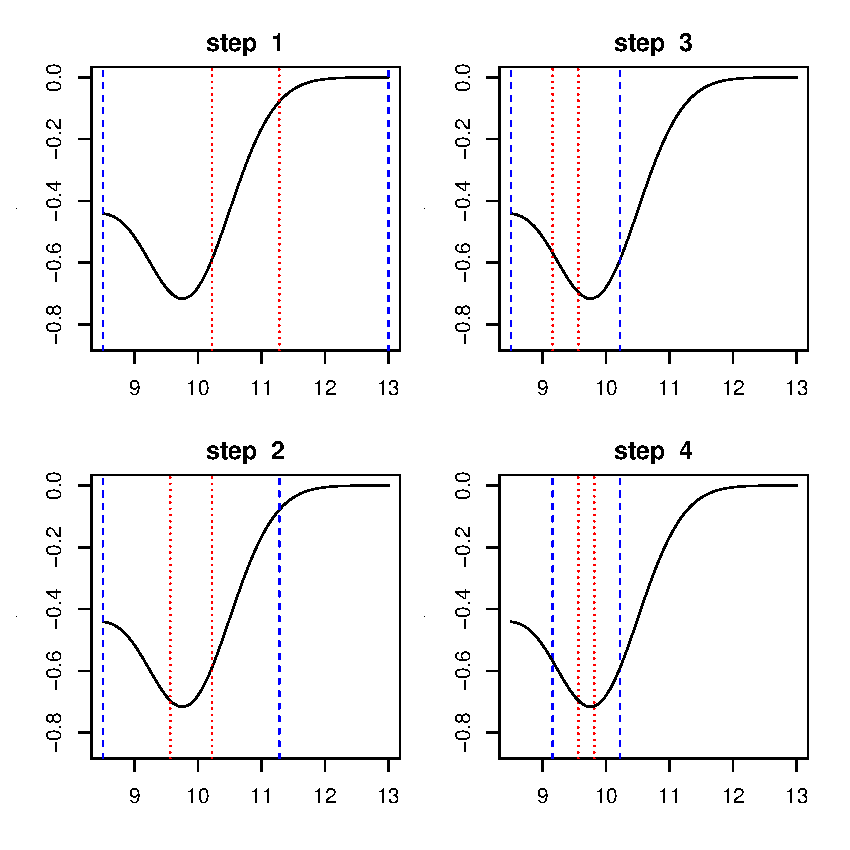
\includegraphics[width=4.0in]
{02Background/goldSecEx01.eps}
\end{center}
\caption{ตัวอย่างการทำค้นหาแบ่งช่วงทองคำ $4$ ขั้นตอน.
ภาพซ้ายบนแสดงขั้น $1$ เส้นแนวตั้งแสดงจุด $a_0$, $a_1$, $b_1$, และ $b_0$.
ภาพซ้ายล่างแสดงขั้น $2$ ช่วงขยับเข้าจากด้านขวา.
ภาพขวาบนแสดงขั้น $3$ ช่วงขยับเข้าจากด้านขวา.
ภาพขวาล่างแสดงขั้น $4$ ช่วงขยับเข้าจากด้านซ้าย.
แต่ละขั้นตอนจะทำให้ช่วงแคบลงเป็น $\approx 0.6$ เท่าของขนาดช่วงก่อนหน้า.
}
\label{fig: golden search example}
\end{figure}
%

\section{วิธีลงเกรเดียนต์}
\label{sec: Gradient Descent}
\index{Gradient Descent Method}
\index{วิธีลงเกรเดียนต์}

\textit{วิธีการค้นหาแบ่งช่วงทองคำ} แม้จะทำงานได้ดี
แต่มีข้อจำกัดที่สำคัญคือ \textit{วิธีการค้นหาแบ่งช่วงทองคำ}เป็นจะทำงานแบบ\textit{การค้นหาตามเส้น} (Line Search).
นั่นคือ \textit{วิธีการค้นหาแบ่งช่วงทองคำ}สามารถทำงานได้เฉพาะกับปัญหาที่ค่าตัวแปรตัดสินใจเป็น\textit{สเกล่าร์}เท่านั้น 
ไม่สามารถทำงานได้กับตัวแปรตัดสินใจที่มีหลายๆมิติ $\mathbf{x} \in \mathbb{R}^D, D > 1$.

วิธีหนึ่งในการแก้ปัญหาการหาค่าน้อยที่สุดที่นิยม เพราะทำงานได้ดี สามารถใช้ได้กับปัญหาที่มีตัวแปรตัดสินใจที่มีหลายมิติ
และเขียนโปรแกรมได้ง่ายมากๆ ก็คือ \textit{วิธีลงเกรเดียนต์}.

วิธีลงเกรเดียนต์ใช้กับ\textit{การหาค่าดีที่สุดแบบไม่มีเงื่อนไข} 
(Unconstrained Optimization)
และอาศัยแนวคิดเดียวกับ\textit{เงื่อนไงจำเปนอันดับแรกสำหรับกรณีภายใน}.
นั่นคือ วิธีลงเกรเดียนต์จะใช้\textit{ค่าเกรเดียนต์ของฟังชั่นเป้าหมายต่อตัวแปรตัดสินใจ}เป็นเครื่องชี้ทาง ในการค้นหาค่าทำน้อยที่สุด โดยพยายามจะค้นหาค่าทำน้อยที่สุด ในทิศทางที่น่าจะเจอจุดที่ค่าเกรเดียนต์เป็นศูนย์.

กล่าวง่ายๆ ทิศทางของเกรเดียนต์(ของฟังชั่นเป้าหมายต่อตัวแปรตัดสินใจ) ณ จุดเริ่มต้นของค่าใดก็ตามของตัวแปรตัดสินใจ  
ก็คือทิศทางที่ หากขยับ(ค่าตัวแปรตัดสินใจ)ออกจาก\textit{จุดค่า}%
\footnote{
จุดค่าที่กล่าวถึงในที่นี้ เป็น\textit{จุดค่า}ใน\textit{ปริภูมิหลายมิติ}.
หลายคนอาจสับสนระหว่างค่าตัวเลขกับจุดค่าใน\textit{ปริภูมิหลายมิติ}.
ค่าตัวเลขหนึ่งค่า เป็นสเกล่าร์ เช่น $x = 16$.
นี้คือ ค่าหนึ่งค่า.
แต่ค่าจุดหนึ่งจุด สำหรับจุดในปริภูมิหลายมิติ เป็นเวคเตอร์ 
เช่น $\mathbf{x} = [255, 150, 0]^T$ แทนสีแดงอมแสด.
ค่า $[255, 150, 0]^T$ นี้ คือค่าแทนหนึ่งจุดในปริภูมิ $3$ มิติของระบบสีแดงเขียวน้ำเงิน เป็นต้น.
}นั้นเล็กน้อยตามทิศของเกรเดียนต์แล้ว
ค่าฟังชั่นเป้าหมายจะเพิ่มขึ้น.
ในทางกลับกัน หากขยับออกจากจุดเดิมเล็กน้อยไปตามทิศตรงข้ามกับเกรเดียนต์แล้ว 
ฟังชั่นเป้าหมาย ณ จุดที่ขยับไปจะมีค่าลดลง.
แล้วถ้าขยับจุดที่พิจารณาไปเรื่อยๆในลักษณะนี้ ในที่สุด ก็จะสามารถขยับลงไปจนถึงจุดของค่าทำน้อยที่สุดได้.
ซึ่งก็นี่คือ แนวคิดของ\textit{วิธีลงเกรเดียนต์} (Gradient Descent Method) ซึ่งเขียนเป็น
สมการปรับค่าของตัวแปรตัดสินได้คือ
\begin{eqnarray}
   \mathbf{x}^{(k+1)} = \mathbf{x}^{(k)} 
   - \alpha_k \nabla g(\mathbf{x}^{(k)})
\label{eq: gradient descent update}   
\end{eqnarray}
โดย $\mathbf{x}^{(k)}$ แทนค่าของตัวแปรตัดสินใจในการคำนวณครั้งที่ $k$,
ค่า $\alpha_k$ มีค่า $>0$ เรียกว่า \textit{ขนาดก้าว} (Step Size).\index{ขนาดก้าว}
โดย ถ้า $\alpha_k$ มีค่าเล็กพอ ก็จะรับประกันได้ว่า ค่าของฟังชั่นเป้าหมายของจุดที่ขยับไปใหม่จะมีค่าน้อยกว่าเดิม $g(\mathbf{x}^{(k+1)}) < g(\mathbf{x}^{(k)})$ หรือ กล่าวอีกอย่างคือ หากค่า\textit{ขนาดก้าว}เล็กพอ วิธีลงเกรเดียนต์รับประกันที่จะลู่เข้าหาค่าทำน้อยที่สุดท้องถิ่น.

\begin{myexample}
จงหาค่าทำน้อยที่สุดของฟังชั่นเป้าหมาย $g(x) = - e^{ - (x-5)^2 }$ ด้วยวิธีลงเกรเดียนต์ 
และให้เริ่มต้นจาก $x^{(0)} = 6.5$ และใช้ค่าขนาดก้าวเป็น $0.5$.
\begin{itemize}
\item อันดับแรก คือการหาเกรเดียนต์ของฟังชั่นเป้าหมาย ซึ่งคือ 
\begin{eqnarray}
   \nabla g(x) &=& 
   \frac{d g(x)}{d x} = 
   - e^{ - (x-5)^2 } \cdot (-2 x + 10).
\nonumber   
\end{eqnarray}
\item คำนวณ (สมการ~\ref{eq: gradient descent update}) ครั้งที่ $k=1$ ได้
\begin{eqnarray}
   x^{(1)} &=& x^{(0)} - (0.5) \cdot \nabla g (x^{(0)})
\nonumber \\
   &=& 6.5 - (0.5) \cdot \nabla g (6.5)  
   = 6.5 - (0.5) \cdot \left(- e^{ - (6.5-5)^2 } \cdot (-2 \cdot (6.5) + 10) \right) 
\nonumber \\   
   &=& 6.3419.
\nonumber   
\end{eqnarray}
\item คำนวณครั้งที่ $2$ ถึง $8$ จะได้
\begin{eqnarray}
   x^{(2)} &=& x^{(1)} - (0.5) \cdot \nabla g (x^{(1)})
\nonumber \\
   &=& 6.3419 - (0.5) \cdot \nabla g (6.3419) = 6.1202
\nonumber \\
   x^{(3)} &=& 6.1202 - (0.5) \cdot \nabla g (6.1202) = 5.8009
\nonumber \\
   x^{(4)} &=& 5.8009 - (0.5) \cdot \nabla g (5.8009) = 5.3792
\nonumber \\
   x^{(5)} &=& 5.0508   
\nonumber \\   
   x^{(6)} &=& 5.0001   
\nonumber \\   
   x^{(7)} &=& 5.0000   
\nonumber \\   
   x^{(8)} &=& 5.0000   
\nonumber
\end{eqnarray}

\item และผลลู่เข้าสู่ $x = 5$ ซึ่งคือคำตอบของฟังชั่นเป้าหมายนี้.
สังเกตุค่าเกรเดียนต์ $\nabla g(5) = 0$ ซึ่งเป็นไปตาม\textit{เงื่อนไงจำเปนอันดับแรกสำหรับกรณีภายใน}.
\end{itemize}

\end{myexample}


การเลือกใช้ค่าขนาดก้าว อาจเลือกใช้ค่าขนาดก้าวเป็นค่าคงที่ทุกๆครั้งของการคำนวณก็ได้ 
แต่หากเลือกค่าขนาดก้าวที่เล็กเกินไป ก็อาจทำให้ต้องทำการคำนวณหลายรอบกว่าที่จะได้ความแม่นยำตามที่ต้องการ.
แต่หากเลือกค่าขนาดก้าวที่ใหญ่เกินไป ก็อาจทำให้ไม่ได้ความแม่นยำตามที่ต้องการ ดังแสดงในสองภาพล่างของรูป~\ref{fig: gradient descent step sizes}
ที่แม้จะทำการคำนวณหลายรอบมากกว่า แต่ก็ยังได้ค่าความแม่นยำแย่กว่ามาก
หรือบางครั้งการใช้ขนาดก้าวที่ใหญ่เกินไปมาก นอกจากจะไม่ได้ค่าความแม่นยำที่ต้องการแล้ว ยังอาจนำไปสู่\textit{การลู่ออก} (Divergence) ด้วย (ดูแบบฝึกหัดท้ายบทข้อ 3).\index{Divergence}

% (คำตอบที่ถูกต้องคือ $x^* = 5$ แต่คำตอบที่ได้จาก step size = 1 คือ $5.01577$ เริ่มที่ $x^{(0)}= 6.5$) หรือ $5.01576$ (เริ่มที่ $x^{(0)}= 4$) แม่นยำถึงแค่ทศนิยมตำแหน่งเดียว เทียบกับค่า $x$ ที่ได้จาก step sizes 0.01 กับ 0.1.

%
\begin{figure}
\begin{center}
\includegraphics[width=5.0in]
{02Background/gdFixedStepSize.eps}
\end{center}
\caption{ตัวอย่างผลจากวิธีลงเกรเดียนต์ด้วยขนาดก้าวค่าต่างๆ.
ทุกภาพทางซ้ายเริ่มที่ $x^{(0)} = 6.5$. 
ทุกภาพทางขวาเริ่มที่  $x^{(0)} = 4$.
จุดเริ่มต้นแสดงด้วยวงกลมสีน้ำเงิน.
ค่า $x$ แต่ละรอบการคำนวณแสดงด้วยจุดสีดำ.
ค่าสุดท้ายที่ได้แสดงด้วยกากบาทสีแดง.}
\label{fig: gradient descent step sizes}
\end{figure}
%

\section{วิธีลงชันที่สุด} 
\label{sec: steepest descent method}
\index{Steepest Descent Method}
\index{วิธีลงชันที่สุด}

จากวิธีลงเกรเดียนต์ แทนที่จะเลือกค่า\textit{ขนาดก้าว}คงที่ค่าใดค่าหนึ่ง
\textit{วิธีลงชันที่สุด} (Steepest Descent Method) พัฒนาวิธีลงเกรเดียนต์ โดยการเลือกใช้ค่า $\alpha_k$ ที่จะทำให้ฟังชั่นเป้าหมายลดลงมากที่สุดในการขยับแต่ละครั้ง.
นั่นคือ
\begin{eqnarray}
   \alpha_k = \arg \min_{\alpha \geq 0} g(\mathbf{x}^{(k)} - \alpha \nabla g(\mathbf{x}^{(k)})).
\end{eqnarray}

%\begin{minipage}{5.5in}
%{\small
%\begin{shaded}
%\paragraph{จากตัวอย่างเดิมของวิธีลงเกรเดียนต์,} 
\begin{myexample}[จากตัวอย่างเดิมของวิธีลงเกรเดียนต์]
หาค่าทำน้อยที่สุดของฟังชั่นเป้าหมาย $g(x) = - e^{ - (x-5)^2 }$ ด้วยวิธีลงชันที่สุด และให้เริ่มจาก $x^{(0)} = 6.5$
\begin{itemize}
\item เกรเดียนต์ $\nabla g(x) = - e^{ - (x-5)^2 } \cdot (-2 x + 10)$.
\item วิธีลงชันที่สุดจะใช้การค้นหาแบ่งช่วงทองคำเพื่อหา
 $\alpha \in [0,1]$ ที่ทำให้ $h(\alpha)$ น้อยที่สุด,
\begin{eqnarray}
  h(\alpha) &=& g(x - \alpha \nabla g(x))
\nonumber \\  
  &=& - \exp \left\{ - (x - \alpha \cdot \left(- e^{ - (x-5)^2 } \cdot (-2 x + 10) \right) -5)^2 \right\}.
  \nonumber
\end{eqnarray} 

%ดังนั้น ตั้ง $a_0 = 0$ และ $b_0 = 1$,
%ดังนั้น 
\item การคำนวณครั้ง $1$, 
\begin{eqnarray}
\alpha_1 = \arg \min_{\alpha \in [0,1]} - \exp \left\{ - (6.5 - \alpha \cdot \left(- e^{ - (6.5-5)^2 } \cdot (-2 (6.5) + 10) \right) -5)^2 \right\}
\nonumber
\end{eqnarray}
 โดยผลจากการค้นหาแบ่งช่วงทองคำได้ $\alpha_1 = 1$
\item ดังนั้น $x^{(1)} = 6.5 - (1) \nabla g(6.5) = 6.1838$.

\item การคำนวณครั้ง $2$, 
\begin{eqnarray}
\alpha_2 = \arg \min_{\alpha \in [0,1]} - \exp \left\{ - (6.1838 - \alpha \cdot \left(- e^{ - (6.1838-5)^2 } \cdot (-2 (6.1838) + 10) \right) -5)^2 \right\}
\nonumber
\end{eqnarray}
 โดยผลจากการค้นหาแบ่งช่วงทองคำได้ $\alpha_2 = 1$
\item ดังนั้น $x^{(2)} = 6.1838 - (1) \nabla g(6.1838) = 5.6008$.

\item การคำนวณครั้ง $3$, 
%\begin{eqnarray}
%\alpha_3 = \arg \min_{\alpha \in [0,1]} - \exp \left\{ - (5.6008 - \alpha \cdot \left(- e^{ - (5.6008-5)^2 } \cdot (-2 (5.6008) + 10) \right) -5)^2 \right\}
%\nonumber
%\end{eqnarray}
% โดย  
ผลจากการค้นหาแบ่งช่วงทองคำได้ $\alpha_3 = 0.7173$
\item ดังนั้น $x^{(3)} = 5.6008 - (0.7173) \nabla g(5.6008) = 4.9997$.

\item การคำนวณครั้ง $4$, 
%\begin{eqnarray}
%\alpha_3 = \arg \min_{\alpha \in [0,1]} - \exp \left\{ - (4.9997 - \alpha \cdot \left(- e^{ - (4.9997-5)^2 } \cdot (-2 (4.9997) + 10) \right) -5)^2 \right\}
%\nonumber
%\end{eqnarray}
% โดย  
ผลจากการค้นหาแบ่งช่วงทองคำได้ $\alpha_4 = 0.5000$
\item ดังนั้น $x^{(4)} = 4.9997 - (0.5) \nabla g(4.9997) = 5.000$.

\item ซึ่งที่ $x = 5$, ค่า $\nabla g(5) = 0$ และผลลู่เข้าค่า $x = 5$ ซึ่งคือคำตอบ.
\end{itemize}

%\end{shaded}
%}%small
%\end{minipage}

\end{myexample}

\paragraph{ธรรมชาติของวิธีลงชันที่สุด.}
รูป~\ref{fig: steepest descent zig zag} แสดงผลการขยับค่าตัวแปรตัดสินใจ ในการคำนวณแต่ละครั้งของวิธีลงชันที่สุด.
ธรรมชาติของวิธีลงชันที่สุดจะให้ผลในลักษณะที่การขยับค่าตัวแปรตัดสินใจแต่ละครั้งจะมีทิศทางตั้งฉากกับทิศทางการขยับเดิม (ดูแบบฝึกหัดท้ายบทข้อ 4).



%\begin{minipage}{6in}
%\begin{shaded}
%\paragraph{ตัวอย่าง.}


%\begin{eqnarray}
%f(\mathbf{x}) &=& - \exp( -\{(\mathbf{x}-\mathbf{v})^T \cdot \mathbf{Z} \cdot (\mathbf{x}-\mathbf{v}) \} )
%\label{eq: gd illus obj f} \\
%
%f(\mathbf{x} = [x_1,x_2]^T) 
%&=& - \exp( -\left\{
%\begin{bmatrix}
%x_1 - v_1 & x_2 - v_2
%\end{bmatrix}
%\cdot  
%\begin{bmatrix}
%z_{11} & z_{12} \\
%z_{21} & z_{22}
%\end{bmatrix}
%\cdot 
%\begin{bmatrix}
%x_1 - v_1 \\
%x_2 - v_2
%\end{bmatrix}
%\right\} )
%\nonumber \\
%
%&=&
%- \exp( -\left\{
%z_{11} (x_1 - v_1)^2 
%+ (z_{12} + z_{21}) (x_1 - v_1) (x_2 - v_2) \right.
%\nonumber \\
%& & 
%\left.
%+ z_{22} (x_2 - v_2)^2
%\right\} )
%\label{eq: gd illus obj f 2-d} \\
%&=&
%- \exp( -\{
%z_{11} (x_1^2 - 2 x_1 v_1 + v_1^2)
%+ (z_{12} + z_{21}) (x_1 x_2 - v_1 x_2 - x_1 v_2 + v_1 v_2)
%+ z_{22} (x_2^2 -2 x_2 v_2 + v_2^2)
%\} )
%\nabla f([x_1, x_2]^T) 
%&=&
%f([x_1, x_2]^T)\cdot
%\begin{bmatrix}
%   -2 z_{11} x_1 - (z_{12} + z_{21}) x_2 + 2 z_{11} v_1  + (z_{12} + z_{21}) v_2 \\
%   -(z_{12} + z_{21}) x_1 - 2 z_{22} x_2 + (z_{12} + z_{21}) v_1 + 2 z_{22} v_2
%\end{bmatrix}
%\nonumber
%\end{eqnarray}

%\end{shaded}
%\end{minipage}


%
\begin{figure}
\begin{center}
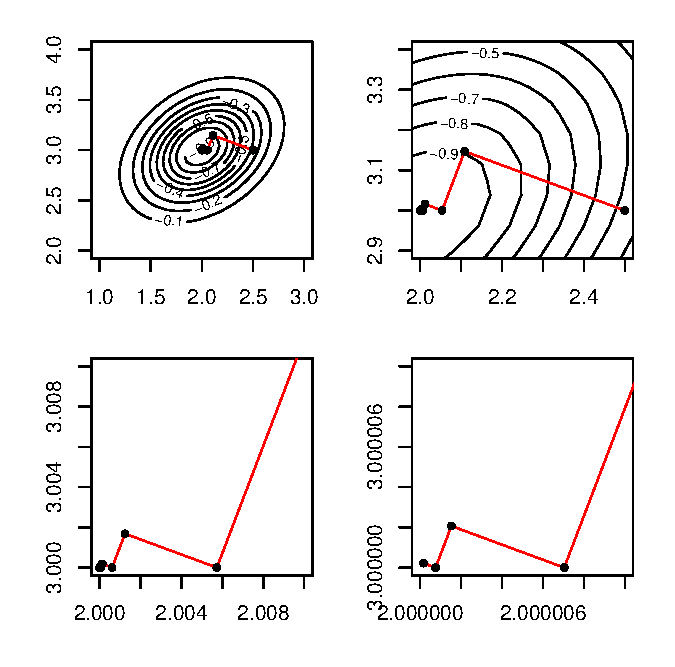
\includegraphics[width=4.0in, height=4.0in]
{02Background/steepestdescentZigZag.eps}
\end{center}
\caption{ผลจากแต่ละการคำนวณของวิธีลงชันที่สุด}
\label{fig: steepest descent zig zag}
\end{figure}
% src: linesearch01a.r



%\subsubsection{Newton Method}

%\subsection{การหาค่าน้อยที่สุดแบบมีข้อจำกัด}
%\label{sec: constraint optimization}

%\paragraph{ปัญหาแบบมีข้อจำกัด (constrained optimization problem)} บ่อยครั้งที่ เซตข้อจำกัดอยู่ในรูป $\Omega = \{ \mathbf{x}: \mathbf{h}(\mathbf{x}) = \mathbf{0}, \mathbf{g}(\mathbf{x}) \le \mathbf{0}\}$

%\section{การคำนวณเชิงวิวัฒนาการ}

%การคำนวณเชิงวิวัฒนาการ (Evolutionary Computation คำย่อ EC)

%จีเนติกอัลกอริทึม (Genetic Algorithm คำย่อ GA)

%\begin{minipage}{5.5in}
%{\small
%\begin{shaded}
%พันธุ์กรรม (Genetics)

%อีพีเจเนติกส์ (Epigenetics)
%\end{shaded}
%}
%\end{minipage}

\section{แบบฝึกหัด}

\paragraph{1.} จงใช้\textit{การค้นหาแบ่งช่วงทองคำ} เพื่อหาค่าทำน้อยที่สุดของฟังชั่นต่อไปนี้
โดยให้ผลลัพธ์แม่นยำขนาดผิดพลาดไม่เกิน $0.0001$

\begin{itemize}
\item ก. $g(x) = (x-5)^2$ โดยเริ่มจากช่วง $x \in [0, 10]$.

\item ข. $g(x) = -0.4 \exp\{-(x-8)^2\}-0.7 \exp\{-(x-9.8)^2\}$ โดยเริ่มจากช่วง $x \in [8.5, 13]$.

\item ค. $g(x) = 2.813 x + 1.843 x^2 -2.187 x^3 + 0.5312 x^4$
โดยเริ่มจากช่วง $x \in [-2, 2]$.
\end{itemize}

โค้ดข้างล่างนี้สำหรับฟังชั่นทำการค้นหาแบ่งช่วงทองคำ 
โดยอาร์กูเมนต์ \texttt{f} แทนฟังชั่นจุดประสงค์
อาร์กูเมนต์ \texttt{a0} และ \texttt{b0} แทนขอบซ้ายและขอบขวาของช่วงที่ต้องการค้นหา
อาร์กูเมนต์ \texttt{tol} แทนค่าความแม่นยำที่ยอมรับได้.

\lstinputlisting[language=R,
caption={การค้นหาแบ่งช่วงทองคำ (Golden Section Search)},
label={lst: golden search}]{02Background/goldensearchCode.r}

ตัวอย่างการใช้งาน เช่น ถ้าฟังชั่นเป้าหมายคือ $g(x) = cos(x)$ และต้องการหาค่า $x$ ในช่วง $x \in [0, 2 \pi]$ โดยให้ค่าผิดพลาดน้อยกว่า $0.001$ ก็สามารถทำได้โดย
\begin{verbatim}
   g <- function(x){ cos(x) }
   results <- goldensearch(g, 0, 2*pi, tol=0.001)
\end{verbatim}
ซึ่งจะได้ผลคือ \texttt{3.141534} ซึ่งตรงกับที่ความรู้เดิมคือโคซายน์ฟังชั่นมีค่าน้อยที่สุดที่ $\pi \approx 3.1416$ และได้ค่าผิดพลาดน้อยกว่า $0.001$.

\paragraph{2.} จากอาร์โค้ดวิธีลงเกรเดียนต์ข้างล่าง จงตอบคำถามข้อ ก. ถึง ง.

\lstinputlisting[language=R,caption={วิธีลงเกรเดียนต์ (Gradient Descent Method)}.
อาร์กูเมนต์ \texttt{x} แทนค่าเริ่มต้นของตัวแปรตัดสินใจ
อาร์กูเมนต์ \texttt{df} แทนเกรเดียนต์ฟังชั่น
อาร์กูเมนต์ \texttt{alpha} แทนค่าขนาดก้าว
อาร์กูเมนต์ \texttt{tol} แทนค่าความแม่นยำที่ยอมรับได้
อาร์กูเมนต์ \texttt{MaXN} แทนจำนวนรอบคำนวณสูงสุด.
โปรแกรมจะหยุดเมื่อได้ค่าความแม่นยำที่ยอมรับได้ หรือครบจำนวนรอบคำนวณสูงสุด ขึ้นกับว่าอะไรถึงก่อน, label={lst: Gradient Descent}]{02Background/graddescentCode.r}

ตัวอย่างเช่น หากต้องการหาค่าทำน้อยที่สุดของฟังชั่น $g(x) = (x-8)^2$, 
(หนึ่ง) หาอนุพันธ์ออกมา เช่น $\nabla g(x) = 2 (x - 8)$,
(สอง) เลือกจุดเริ่มต้น และค่าขนาดก้าว $\alpha$ เช่น ให้ $x^{(0)} = 0$ และ $\alpha = 0.3$
และรัน
\begin{verbatim}
  df <- function(x){ 2 * (x-8) }
  
  results <- gd(x=0, df, alpha=0.3)
\end{verbatim}
ผลลัพธ์ใน \texttt{results} จะเก็บค่า $x$ ในแต่ละการคำนวณ โดยค่าสุดท้ายคือคำตอบที่ได้ เช่น
\begin{verbatim}
> results
 [1] 4.800000 6.720000 7.488000 7.795200 7.918080 7.967232 7.986893 7.994757
 [9] 7.997903 7.999161 7.999664 7.999866 7.999946 7.999979 7.999991 7.999997
\end{verbatim}
คำตอบที่ได้คือ \texttt{7.999997} ซึ่งผิดจากคำตอบที่ถูกต้อง $x^* = 8$ น้อยกว่า $0.00001$ (หรือ $1\times10^5$ ตามที่ระบุไว้ด้วย \texttt{tol})

จงใช้วิธีลงเกรเดียนต์ ตอบคำถามข้างล่าง
\begin{itemize}
\item ก. หาค่าทำน้อยที่สุดของฟังชั่น $f(x) = - \exp\{ - (x - 7)^2 \}$ เริ่มต้นที่ $5.5$ และ ใช้ $\alpha = 0.3$.

\item ข. หาค่าทำน้อยที่สุดของฟังชั่น $h(\mathbf{x} = [x_1, x_2]^T) = (2 x_1 - 9)^2 + (x_2 - 8)^2$ โดยให้เลือกจุดเริ่มต้น และค่า $\alpha$ เอง.

\item ค. ทำข้อ ก. ใหม่โดยเปลี่ยนค่าเริ่มต้น เป็น $2$ และอธิบายว่าเกิดอะไรขึ้น

\item ง. ทำข้อ ก. ใหม่โดยใช้ค่าเริ่มต้นที่ $5.5$ และหาค่า $\alpha$ ที่ทำให้ลู่เข้าได้เร็วที่สุด.


\end{itemize}


\paragraph{3.} จงใช้วิธีลงเกรเดียนต์เพื่อหาค่าทำน้อยที่สุดของฟังชั่นที่กำหนดดังอาร์โค้ดข้างล่าง
\begin{verbatim}
   w <- c(1.827579e-14, 2.812698e+00, 1.843386e+00,
       -2.187302e+00, 5.312169e-01)

   f <- function(x){ 
      w[1] + w[2]*x + w[3]*x^2 + w[4]*x^3 + w[5]*x^4
   }
\end{verbatim}
ใช้ค่าเริ่มต้นที่ $x^{(0)} = 2$ แต่ทดลองค่า $\alpha$ เป็น $0.1$ กับ $1$ และได้ผลดังแสดงในรูป~\ref{fig: gd large step size diverge}.
ตอนที่ใช้ค่าขนาดก้าวเป็น $0.1$ วิธีลงเกรเดียนต์ทำการคำนวณไป $21$ ครั้งแล้วได้ผลลัพธ์เป็น $-0.41507$.
ตอนที่ใช้ค่าขนาดก้าวเป็น $1$ วิธีลงเกรเดียนต์ทำการคำนวณแค่ $9$ ครั้งแล้วได้ผลลัพธ์เป็น $\infty$, ซึ่งไม่ถูกต้อง.
พอนำค่าตัวแปรตัดสินใจที่ขยับแต่ละการคำนวณมาวาดกราฟ ดังแสดงในภาพขวาล่าง (รูป~\ref{fig: gd large step size diverge}) 
อธิบายว่าเกิดอะไรขึ้น ทำไมจึงมีค่าของตัวแปรตัดสินใจที่อยู่ใกล้คำตอบแล้วจึงวิ่งออกห่างไป.

%
\begin{figure}
\begin{center}
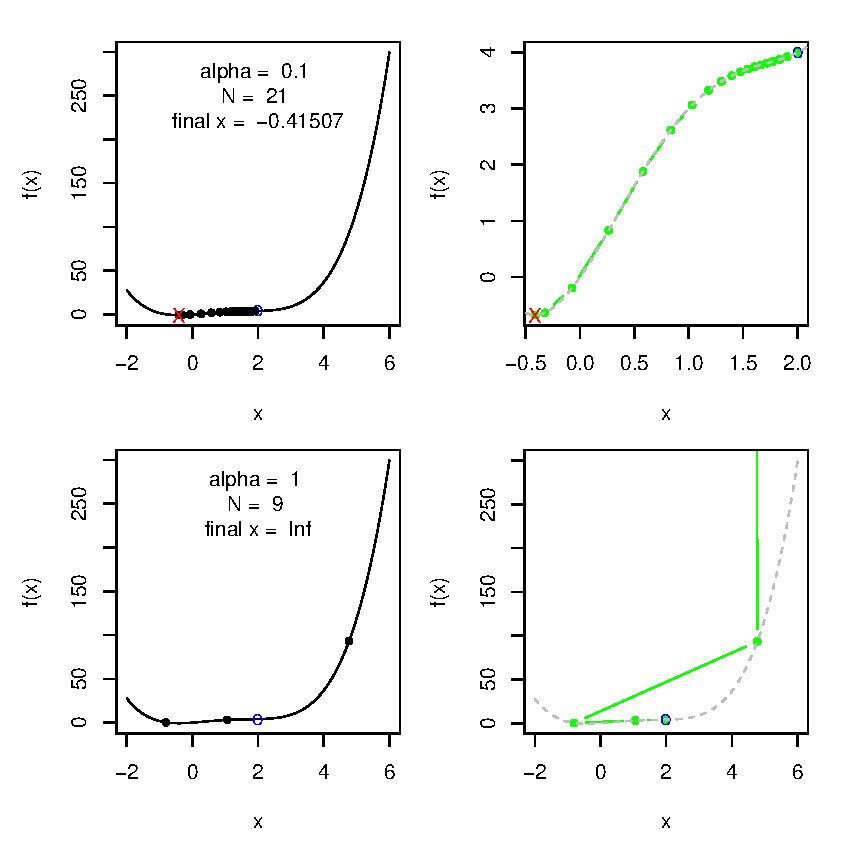
\includegraphics[width=6.0in]
{02Background/gdStepSizeDiverge.eps} 
\end{center}
\caption{แบบฝึกหัดข้อ 13. สองภาพบนแสดงผลจากการคำนวณแต่ละครั้งของวิธีลงเกรเดียนต์ที่ใช้ $\alpha = 0.1$.
สองภาพล่างแสดงผลจากการใช้ $\alpha = 1$.
โดย ภาพทางซ้ายแสดงภาพรวม ค่าเริ่มต้น (แทนด้วยวงกลม) ค่าสุดท้าย (แทนด้วยกากบาท) ค่าที่ได้จากผลจากการคำนวณแต่ละครั้ง (แทนด้วยจุดสีดำ) และผลสรุปซึ่งเขียนไว้บริเวณกลางภาพ
และภาพขวาขยายให้เห็นเส้นทางการขยับของค่าตัวแปรตัดสินใจจากการคำนวณแต่ละครั้ง.
ผลสรุปที่กลางภาพ ของสองภาพซ้าย คือ ค่าขนาดก้าว จำนวนรอบการคำนวณที่ทำ ค่าตัวแปรตัดสินใจค่าสุดท้ายที่ได้ ตามลำดับจากบนลงล่าง}
\label{fig: gd large step size diverge}
\end{figure}
% src: linesearch01a.r

\paragraph{4.} 
จากอาร์โค้ดข้างล่างทำวิธีลงชันที่สุด จงหาค่าทำน้อยที่สุดของฟังชั่น ข้อ ก. ถึง ง.
\lstinputlisting[language=R, caption={วิธีลงชันที่สุด (Steepest Descent Method).
อาร์กูเมนต์ \texttt{grad} แทนเกรเดียนต์ฟังชั่น
อาร์กูเมนต์ \texttt{f} แทนฟังชั่นจุดประสงค์
อาร์กูเมนต์ \texttt{x0} แทนค่าเริ่มต้นของตัวแปรตัดสินใจ
อาร์กูเมนต์ \texttt{tol} แทนค่าความแม่นยำที่ยอมรับได้
อาร์กูเมนต์ \texttt{MaxN} แทนจำนวนรอบคำนวณสูงสุด.
โปรแกรมจะหยุดคำนวณเมื่อได้ค่าความแม่นยำที่ยอมรับได้ หรือถึงจำนวนรอบคำนวณสูงสุด
ขึ้นกับว่าอะไรถึงก่อน
}, label={lst: steepest descent}]{02Background/steepestdescentCode.r}

ตัวอย่าง เช่นถ้าหากต้องการหาค่าทำน้อยที่สุดของ $f(\mathbf{x} = [x_1, x_2]^T) = (x_1 - 3)^2 + (x_2 - 5)^2$ สามารถทำได้โดย (หนึ่ง) หาอนุพันธ์ของฟังชั่นเป้าหมาย(สอง) กำหนดจุดเริ่มต้น เช่น อาจเลือกจุด $[4, 5]^T$ เป็นจุดเริ่มต้น และรันฟังชั่น \texttt{steepestdescent} ดังข้างล่าง
\begin{verbatim}
  f <- function(x){ (x[1] - 3)^2 + (x[2] - 5)^2 }
  df <- function(x){ matrix(c(2*(x[1] -3), 2*(x[2] - 5)),2,1) }

  results <- steepestdescent(df, f, x0=matrix(c(4,5),2,1), log=TRUE)
\end{verbatim}
โค้ดข้างต้น \texttt{f} และ \texttt{df} กำหนดฟังชั่นเป้าหมายและอนุพันธ์ตามลำดับ.

ผล \texttt{results} ที่ได้คือ
\begin{verbatim}
     [,1]     [,2]     [,3]
[1,]    0 1.000000 2.000000
[2,]    0 0.499999 0.499999
[3,]    4 3.000002 3.000000
[4,]    5 5.000000 5.000000
\end{verbatim}
โดยแต่ละคอลัมน์คือ การคำนวณแต่ละครั้ง แถวแรกบอกว่าเป็นการคำนวณครั้งที่เท่าไร (ค่าเริ่มต้น นับเป็นการคำนวณครั้งที่ $0$), แถวที่สองบอกค่า $\alpha$ ที่ใช้, แถวต่อๆมาเป็นค่าของตัวแปรตัดสินใจ เช่น 
จากผลข้างต้น \texttt{steepestdescent} ทำการคำนวณ $2$ ครั้ง
โดย
ครั้งที่ 1 ใช้ $\alpha = 0.499999$ และได้ขยับค่าตัวแปรไปเป็น \texttt{3.000002} กับ \texttt{5.000000}
และครั้งที่ 2 ก็ใช้ $\alpha = 0.499999$ และได้ขยับค่าตัวแปรไปเป็น $3$ กับ $5$ ซึ่งคือคำตอบ.

\begin{itemize}
\item ก. จงหาค่าทำน้อยที่สุดของ $h([x_1, x_2]^T) = -\exp(-(x_1 - 7)^2) + (x_2 - 4)^2$ โดยใช้ $[0, 0]^T$ เป็นค่าเริ่มต้น.

\item ข. จงหาค่าทำน้อยที่สุดของ $g(x) = x^2 + 4 x + 15$ โดยใช้ $15$ เป็นค่าเริ่มต้น.

\item ค. จงหาค่าทำน้อยที่สุดของ $f(\mathbf{x} = [x_1, x_2]^T) =
- \exp( -\{
z_{11} (x_1^2 - 2 x_1 v_1 + v_1^2)
+ (z_{12} + z_{21}) (x_1 x_2 - v_1 x_2 - x_1 v_2 + v_1 v_2)
+ z_{22} (x_2^2 -2 x_2 v_2 + v_2^2)
\} )$ 
โดย $v_1 = 2$, $v_2 = 3$, $z_{11} = 4$, $z_{12} = z_{21} = -1.5$, $z_{22} = 5$, และ ใช้ค่าเริ่มต้นเป็น $[2.5,3]^T$ เสร็จแล้ววาดรูปแบบรูป~\ref{fig: steepest descent zig zag}.
[คำใบ้: ลอง \texttt{help(contour)}]

\item ง. ทำข้อ ค. อีกครั้งโดยสุ่มค่าเริ่มต้น เสร็จแล้ววาดรูปแบบเดียวกับ ค.
[คำใบ้: ลอง \texttt{help(rnorm)}]

\end{itemize}






